\chapter{基因和行为} \label{chap:chap2}

所有行为都是由基因和环境的相互作用塑造的。
简单动物的大多数刻板行为都受到环境的影响,而人类高度进化的行为则受到基因指定的先天特性的限制。
基因不直接控制行为,但基因编码的\textit{核糖核酸}和蛋白质会在不同时间和多个层面发挥作用,影响大脑。
基因指定了组装大脑的发育程序,并且对于神经元、神经胶质细胞和突触的特性至关重要,这些特性使神经元回路发挥作用。
代代稳定遗传的基因创造了新体验可以在学习过程中改变大脑的机制。


在本章中,我们将探讨基因如何影响行为。
我们首先概述基因确实影响行为的证据,然后回顾分子生物学和遗传传递的基本原理。
然后,我们提供了遗传对行为影响的记录方式的示例。
通过对蠕虫、苍蝇和老鼠的研究,人们对基因调节行为的方式有了深刻的了解,这些动物的基因组可用于实验操作。
通过对人类大脑发育和功能的分析,基因和人类行为之间出现了许多有说服力的联系。
尽管研究人类复杂特征存在固有的巨大挑战,但最近的进展已经开始揭示神经发育和精神综合征(如自闭症、精神分裂症和双相情感障碍)的遗传风险因素,为阐明基因、大脑和行为。



\section{了解分子遗传学和遗传率对于研究人类行为至关重要}

许多人类精神疾病和神经系统疾病都有遗传因素。
患者的亲属比一般人群更容易患上这种疾病。
遗传因素对群体特性的影响程度称为\textit{遗传力}。
遗传力最强的案例是基于双胞胎研究,1883 年\textit{弗朗西斯·高尔顿}首次使用了同卵双胞胎。
这样的同卵双胞胎共享所有基因。
相反,异卵双胞胎是由两个不同的受精卵发育而来的;
这些异卵双胞胎与正常的兄弟姐妹一样,平均共享一半的遗传信息。
多年来的系统比较表明,同卵双胞胎在神经和精神特征方面往往比异卵双胞胎更相似(一致),这为这些特征的可遗传成分提供了证据(图~\ref{fig:2_1}A)。


\begin{figure}[htbp]
	\centering
	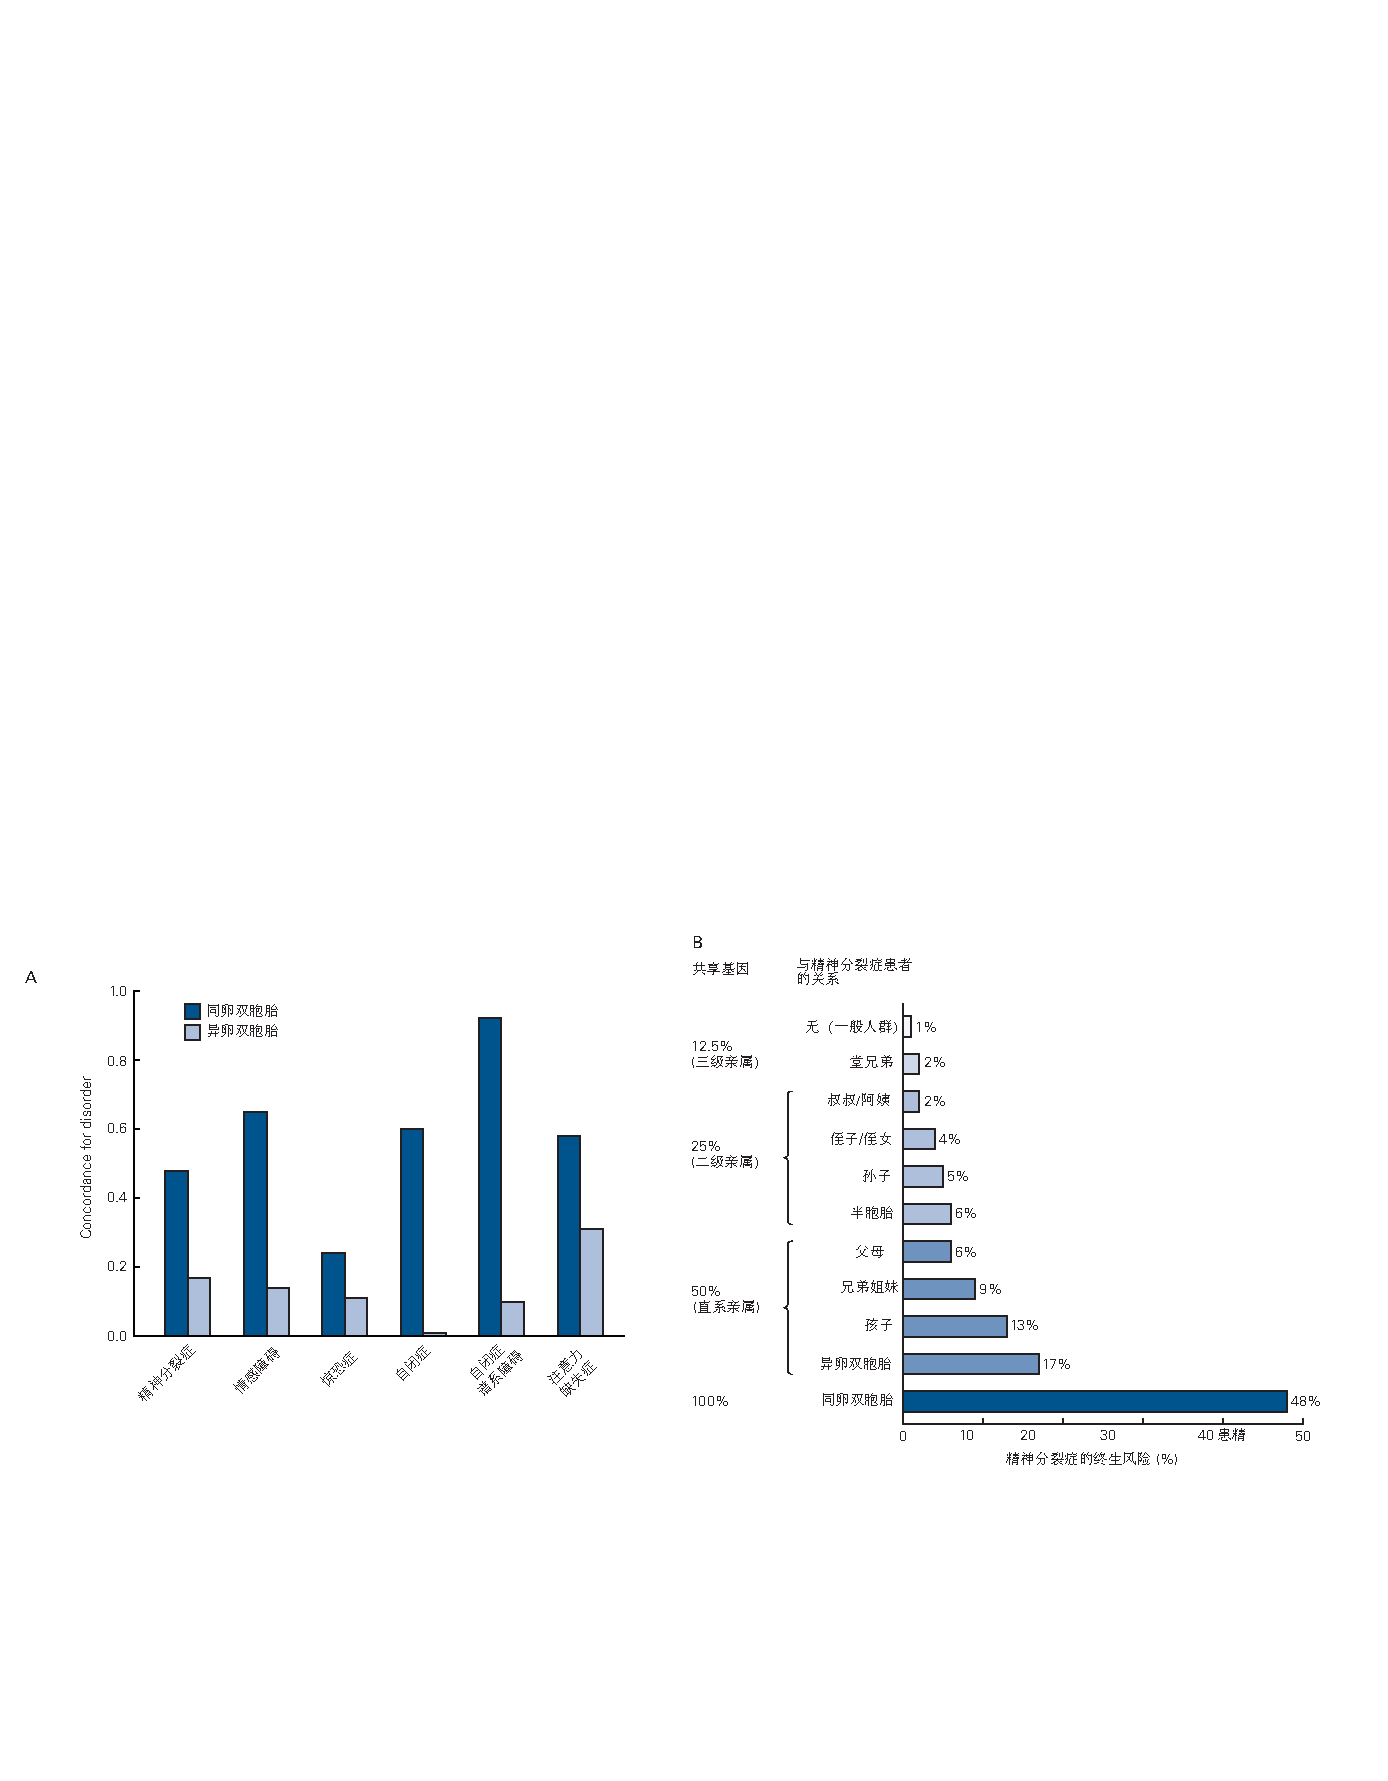
\includegraphics[width=0.9\linewidth]{chap02/fig_2_1}
	\caption{精神疾病的家族风险提供了遗传性的证据。
		A. 同卵双胞胎之间精神疾病的相关性比异卵双胞胎之间的相关性大得多。
		同卵双胞胎几乎共享所有基因,并且有很高(但不是 100\%)共享疾病状态的风险。
		异卵双胞胎共享 50\% 的遗传物质。
		零分表示没有相关性(两个随机人的平均结果),而 1.0 分表示完全相关\cite{mcgue1998genetic}。
		B. 精神分裂症患者的近亲患精神分裂症的风险更大。
		就像异卵双胞胎一样,父母和孩子以及兄弟姐妹共享 50\% 的遗传物质。
		如果只有一个基因导致精神分裂症,那么患者的父母、兄弟姐妹、孩子和异卵双胞胎的风险应该是相同的。 
		家庭成员之间的差异表明更复杂的遗传和环境因素在起作用\cite{gottesman1991schizophrenia}。}
	\label{fig:2_1}
\end{figure}


在双胞胎研究模型的一个变体中,明尼苏达双胞胎研究调查了在生命早期分开并在不同家庭中长大的同卵双胞胎。
尽管有时环境差异很大,但双胞胎对相同的精神疾病有着共同的倾向,甚至倾向于共享性格特征,比如外向性。
这项研究提供了大量证据,证明遗传变异会导致正常的人类差异,而不仅仅是疾病状态。


人类疾病和行为特征的遗传率通常大大低于 100\%,表明环境是获得疾病或特征的重要因素。
如图~\ref{fig:2_1}B~所示,来自双胞胎研究的许多神经学、精神病学和行为特征的遗传力估计值约为 50\%,但特定特征的遗传力可能更高或更低。
尽管对同卵双胞胎和其他亲属关系的研究支持人类行为具有遗传成分的观点,但它们并没有告诉我们哪些基因是重要的,更不用说特定基因如何影响行为了。
这些问题通过对实验动物的研究得到解决,其中遗传和环境因素受到严格控制,并通过现代基因发现方法得到解决,这些方法现在可以系统、可靠地识别\textit{脱氧核糖核酸}序列和结构中的特定变异,这些变异促成人类精神病学和神经学的表现型。



\section{对基因组结构和功能的理解正在演变}

分子生物学和传递遗传学的相关领域是我们现代对基因的理解的核心。
在这里,我们总结了这些领域的一些关键思想;
本章末尾的词汇表定义了常用术语。


基因由\textit{脱氧核糖核酸}组成,\textit{脱氧核糖核酸}代代相传。
在大多数情况下,每个基因的精确拷贝都会提供给生物体中的所有细胞,并通过\textit{脱氧核糖核酸}复制提供给后代。
该一般规则的罕见例外——引入种系或体细胞\textit{脱氧核糖核酸}并在疾病风险中发挥重要作用的新(从头)突变——将在后面讨论。
\textit{脱氧核糖核酸}由两条链组成,每条链都有一个脱氧核糖磷酸骨架连接到一系列四个亚基:核苷酸\textit{腺嘌呤}、\textit{鸟嘌呤}、\textit{胸腺嘧啶}和\textit{胞嘧啶}。
如图~\ref{fig:2_2}~所示,两条链配对,一条链上的\textit{腺嘌呤}总是与互补链上的\textit{胸腺嘧啶}配对,\textit{鸟嘌呤}与\textit{胞嘧啶}配对。
这种互补性确保了\textit{脱氧核糖核酸}复制过程中\textit{脱氧核糖核酸}的准确复制,并驱动\textit{脱氧核糖核酸}转录成称为转录本的\textit{核糖核酸}长度。
鉴于几乎所有的基因组都是双链的,碱基或碱基对可以互换使用作为测量单位。
包含一千个碱基对的基因组片段称为 1 千碱基 (1 kb) 或 1 千碱基对 (1 kbp),而一百万碱基对称为 1 兆碱基 (1 Mb) 或 1 兆碱基对 (1 Mbp)。
\textit{核糖核酸}与\textit{脱氧核糖核酸}的不同之处在于\textit{核糖核酸}是单链的,具有核糖而不是脱氧核糖骨架,并使用核苷碱基\textit{尿苷}代替\textit{胸腺嘧啶}。


\begin{figure}[htbp]
	\centering
	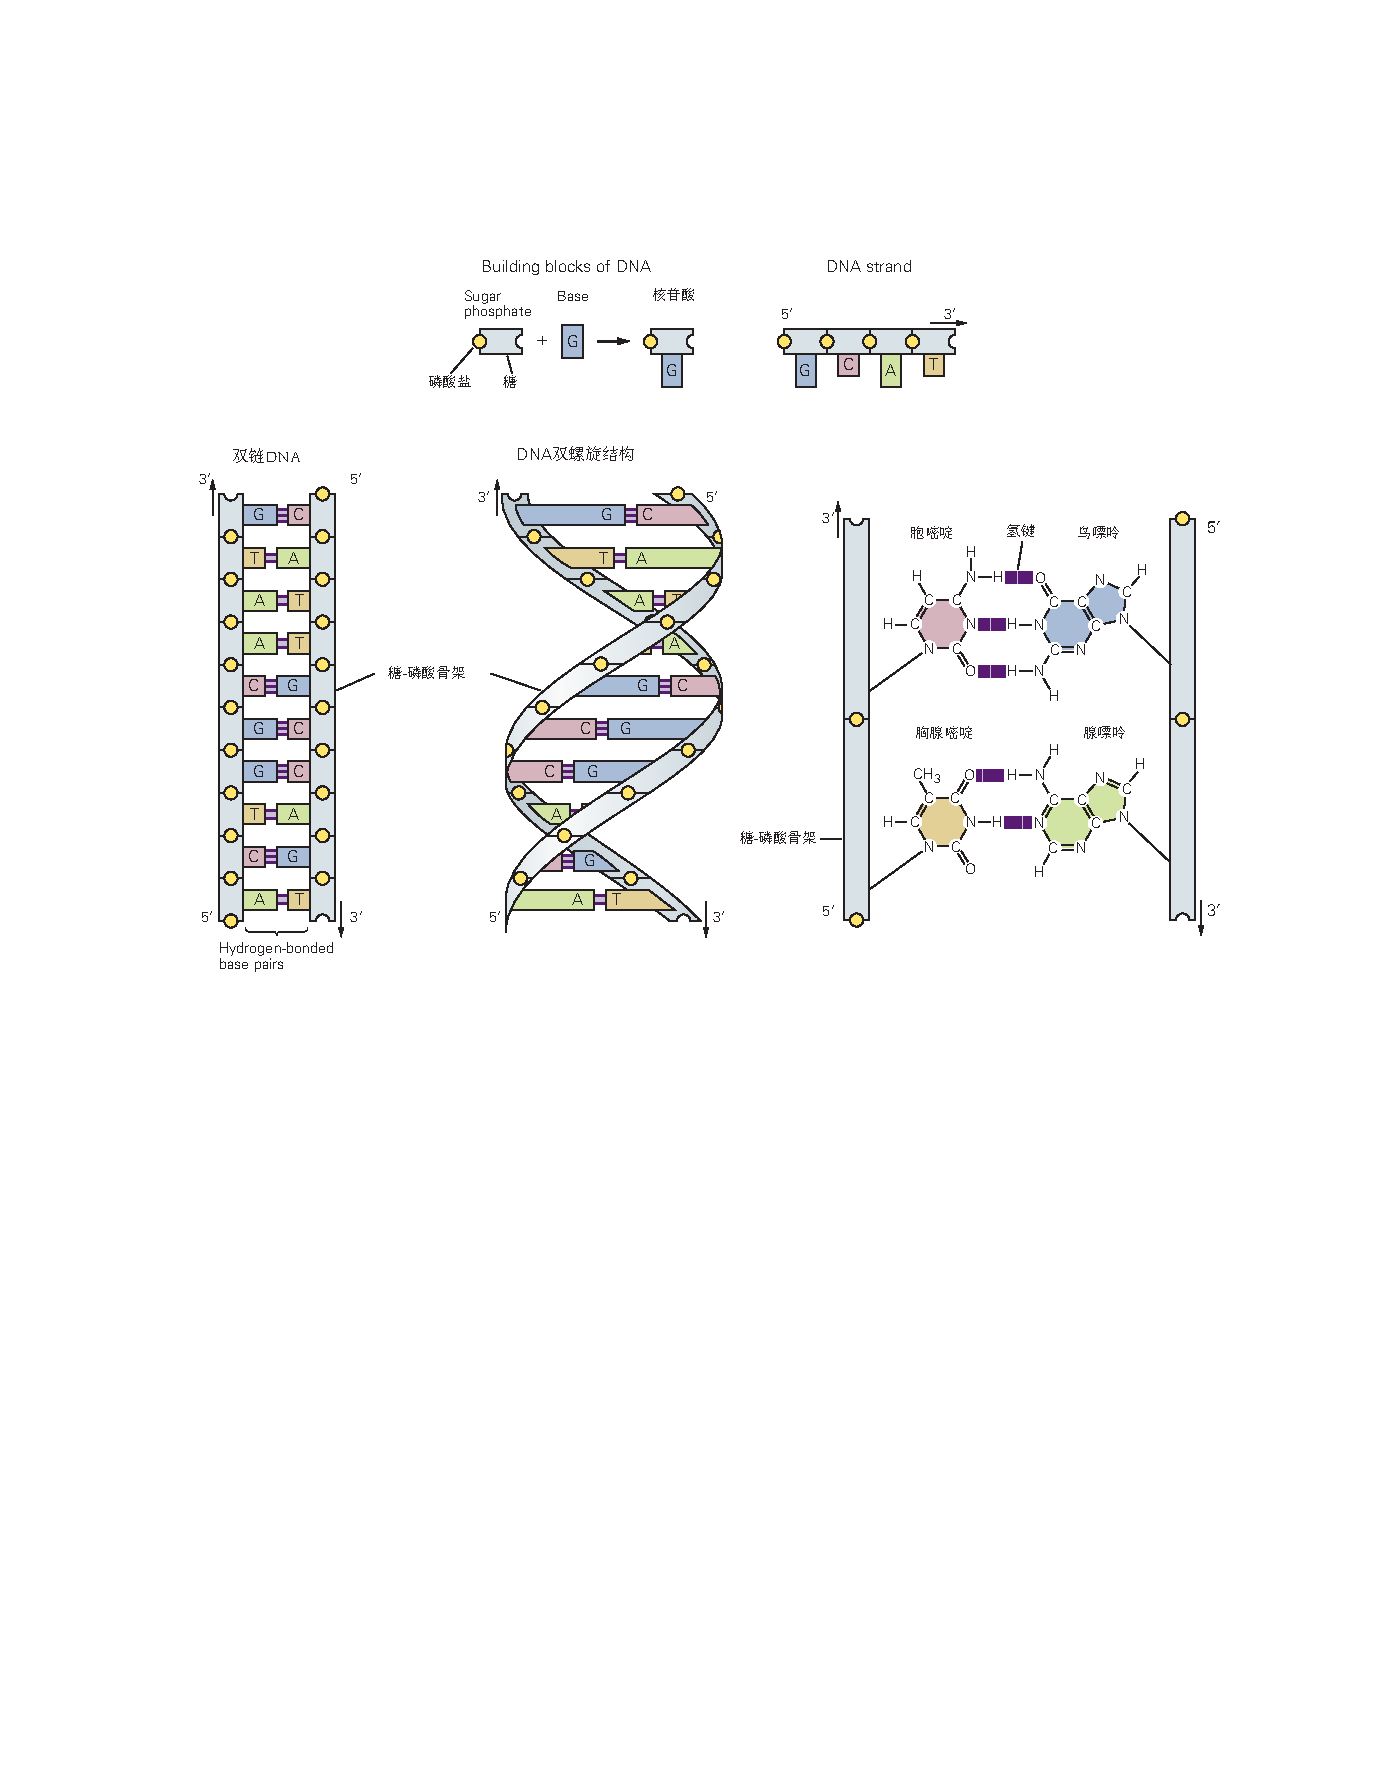
\includegraphics[width=0.5\linewidth]{chap02/fig_2_2}
	\caption{\textit{脱氧核糖核酸}的结构。
		四种不同的核苷酸碱基,腺嘌呤 (A)、胸腺嘧啶 (T)、胞嘧啶 (C) 和鸟嘌呤 (G),组装在双链\textit{脱氧核糖核酸}螺旋的糖磷酸主链上\cite{alberts2017molecular}。}
	\label{fig:2_2}
\end{figure}


在人类基因组中,大约有 2 万个基因编码蛋白质产物,这些蛋白质产物是通过将线性\textit{信使核糖核酸}序列翻译成由氨基酸组成的线性多肽(蛋白质)序列而产生的。
一个典型的蛋白质编码基因由一个编码区和非编码区组成,编码区被翻译成蛋白质(图~\ref{fig:2_3})。
编码区通常排列在称为外显子的小编码区段中,它们被称为内含子的非编码区隔开。
在翻译成蛋白质之前,内含子从\textit{信使核糖核酸}中删除。


\begin{figure}[htbp]
	\centering
	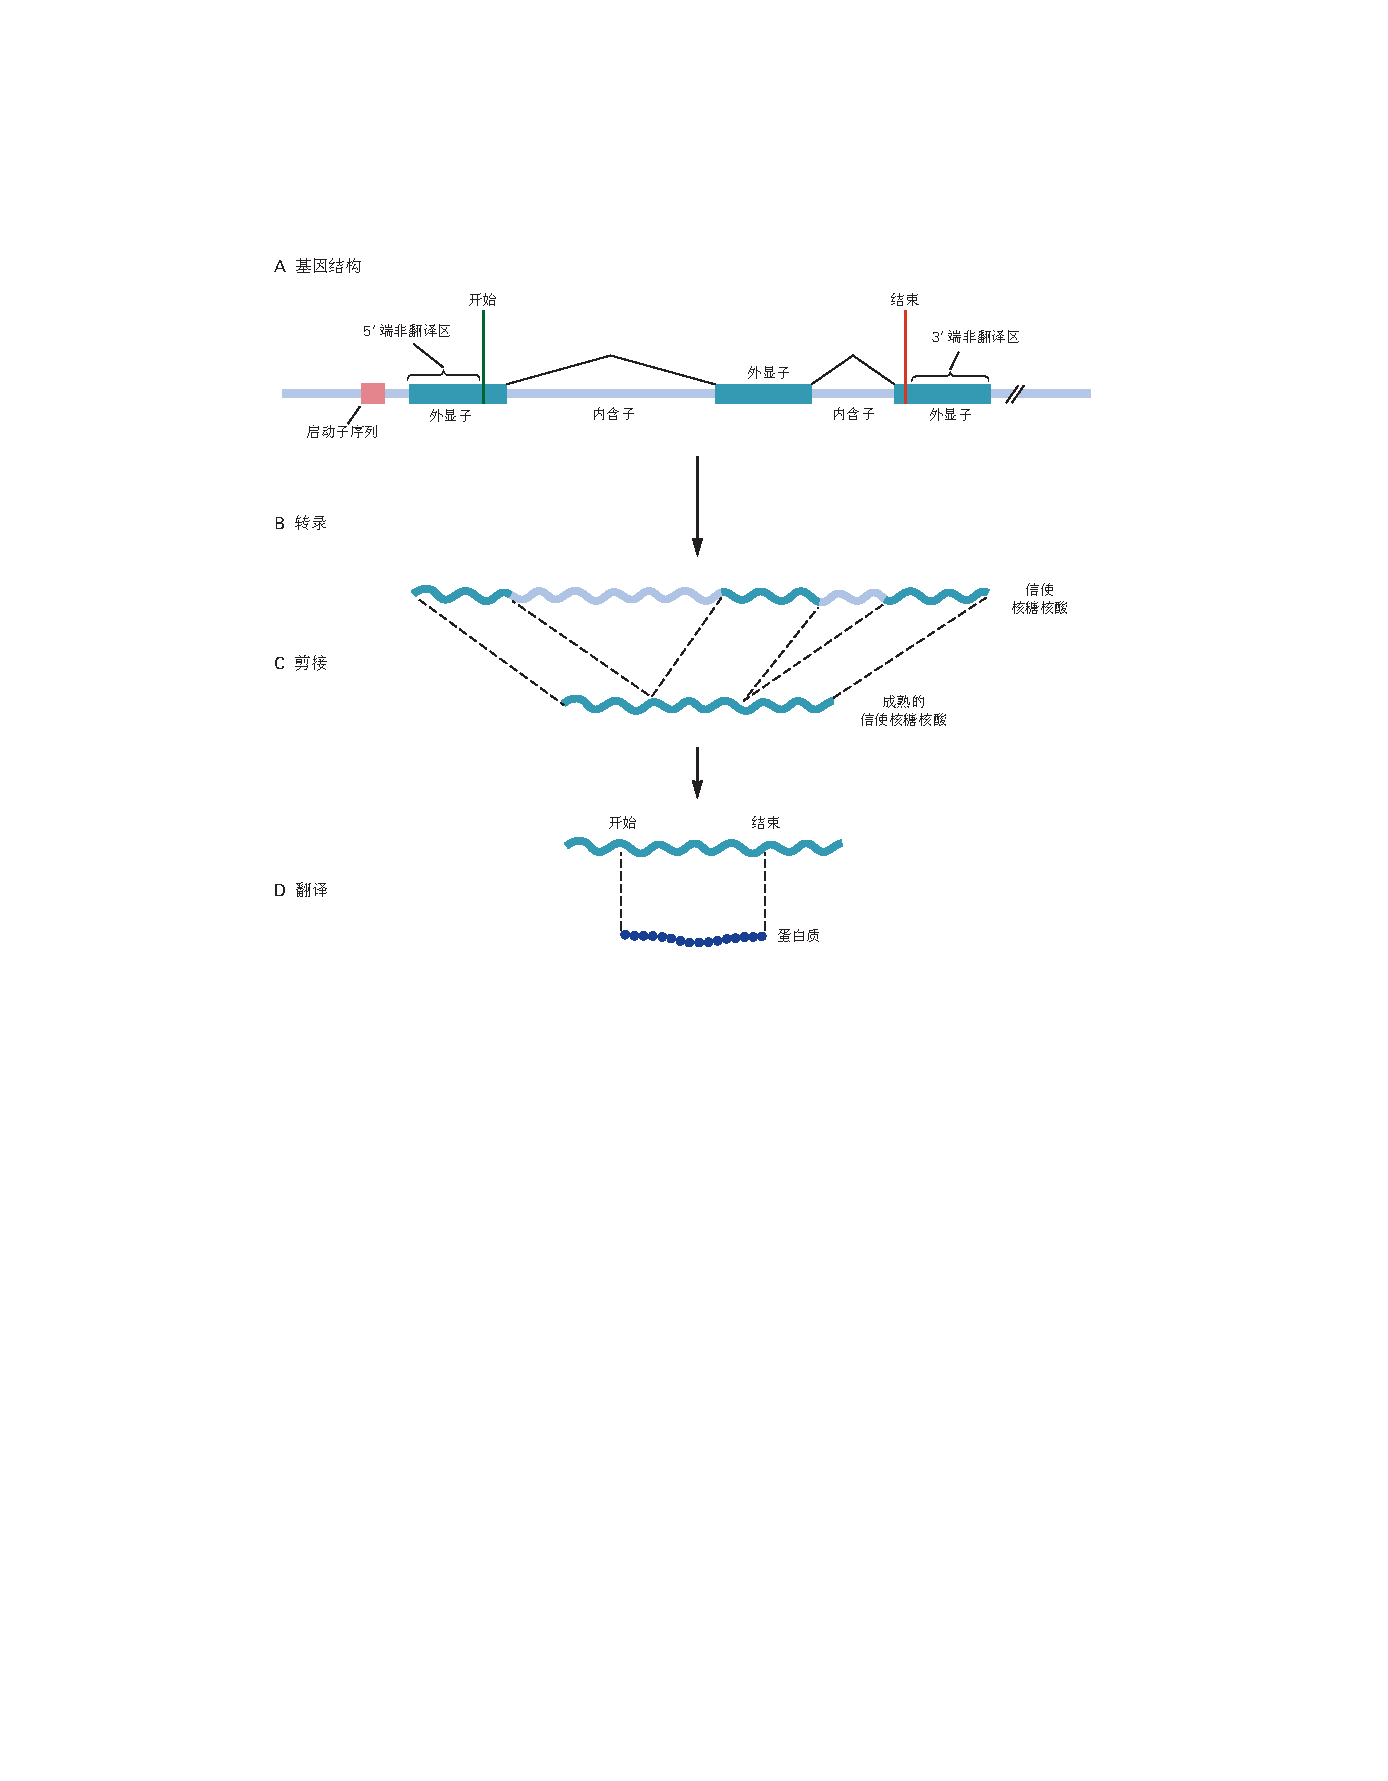
\includegraphics[width=0.5\linewidth]{chap02/fig_2_3}
	\caption{基因结构和表达。
		\textbf{A.} 一个基因由被非编码区(内含子)隔开的编码区(外显子)组成。
		它的转录受非编码区调节,例如经常在基因开始附近发现的启动子和增强子。
		\textbf{B.} 转录导致产生包括外显子和内含子的初级单链\textit{核糖核酸}转录物。
		\textbf{C.} 剪接从未成熟的转录物中去除内含子,并将外显子连接成成熟的\textit{信使核糖核酸},后者从细胞核输出。
		\textbf{D.} 成熟\textit{信使核糖核酸}的翻译产生蛋白质产物。}
	\label{fig:2_3}
\end{figure}


许多功能性\textit{核糖核酸}转录物不编码蛋白质。 
事实上,在人类基因组中,与大约 20,000 个蛋白质编码基因相比,已经表征了超过 40,000 个非编码转录本。
这些基因包括\textit{核糖体核糖核酸}和\textit{转运核糖核酸},它们是\textit{信使核糖核酸}翻译机制的重要组成部分。
其他\textit{非编码核糖核酸}包括\textit{长链非编码核糖核酸},任意定义为长度超过 200 bp,不编码蛋白质但可以在基因调控中发挥作用;
指导\textit{信使核糖核酸}剪接的多种类型的\textit{小非编码核糖核酸},包括\textit{小核核糖核酸};
和与特定\textit{信使核糖核酸}中的互补序列配对以抑制其翻译的\textit{微小核糖核酸}。


身体中的每个细胞都包含每个基因的\textit{脱氧核糖核酸},但仅将基因的特定子集表达为\textit{核糖核酸}。
转录成\textit{核糖核酸}的基因部分两侧是非编码\textit{脱氧核糖核酸}区域,这些区域可能与其他蛋白质(包括转录因子)结合以调节基因表达。
这些序列基序包括启动子、增强子、沉默子和绝缘子,它们一起允许\textit{核糖核酸}在正确的时间在正确的细胞中准确表达。
启动子通常位于待转录区域的开头附近;
增强子、消音子和绝缘子可能与被调节的基因存在一定距离。
每种类型的细胞都有独特的\textit{脱氧核糖核酸}结合蛋白补充,这些蛋白与启动子和其他调节序列相互作用,以调节基因表达和由此产生的细胞特性。


大脑表达的基因数量比身体的任何其他器官都要多,而且在大脑内,不同的神经元群表达不同的基因组。
由启动子、其他调节序列和与其相互作用的\textit{脱氧核糖核酸}结合蛋白控制的选择性基因表达允许固定数量的基因在大脑中产生数量大得多的神经元细胞类型和连接。


虽然基因指定了神经系统的初始发育和特性,但个体的经历和特定神经回路中由此产生的活动本身可以改变基因的表达。
通过这种方式,环境影响被纳入神经回路的结构和功能。
基因研究的一些主要目标是阐明单个基因影响生物过程的方式、基因网络影响彼此活动的方式以及基因与环境相互作用的方式。



\subsection{基因排列在染色体上}

细胞中的基因有序地排列在称为染色体的长而线性的\textit{脱氧核糖核酸}上。
人类基因组中的每个基因都可重复地位于特定染色体上的特征位置(\textit{基因座}),并且该遗传“地址”可用于将生物学特征与基因的作用相关联。
大多数多细胞动物(包括蠕虫、果蝇和小鼠,以及人类)都是二倍体;
每个体细胞都携带两套完整的染色体,一套来自母亲,另一套来自父亲。


人类有大约 2 万个基因,但只有 46 条染色体:22 对常染色体(男性和女性都存在的染色体)和两条性染色体(女性有两条 X 染色体,男性有一条 X 染色体和一条 Y 染色体)(图~\ref{fig:2_4})。
每个父母都向二倍体后代提供每个常染色体的一个副本。
每个父母也为女性 (XX) 后代提供一条 X 染色体,但 XY 男性从母亲那里继承了一条 X 染色体,从父亲那里继承了一条 Y 染色体。
1910 年,\textit{摩尔根}在果蝇身上发现了\textit{伴性遗传}。
这种与单个 X 染色体相关的\textit{伴性遗传}模式在人类遗传学研究中非常重要,某些 X 连锁遗传病通常仅在男性,但基因会从母亲传给儿子。


\begin{figure}[htbp]
	\centering
	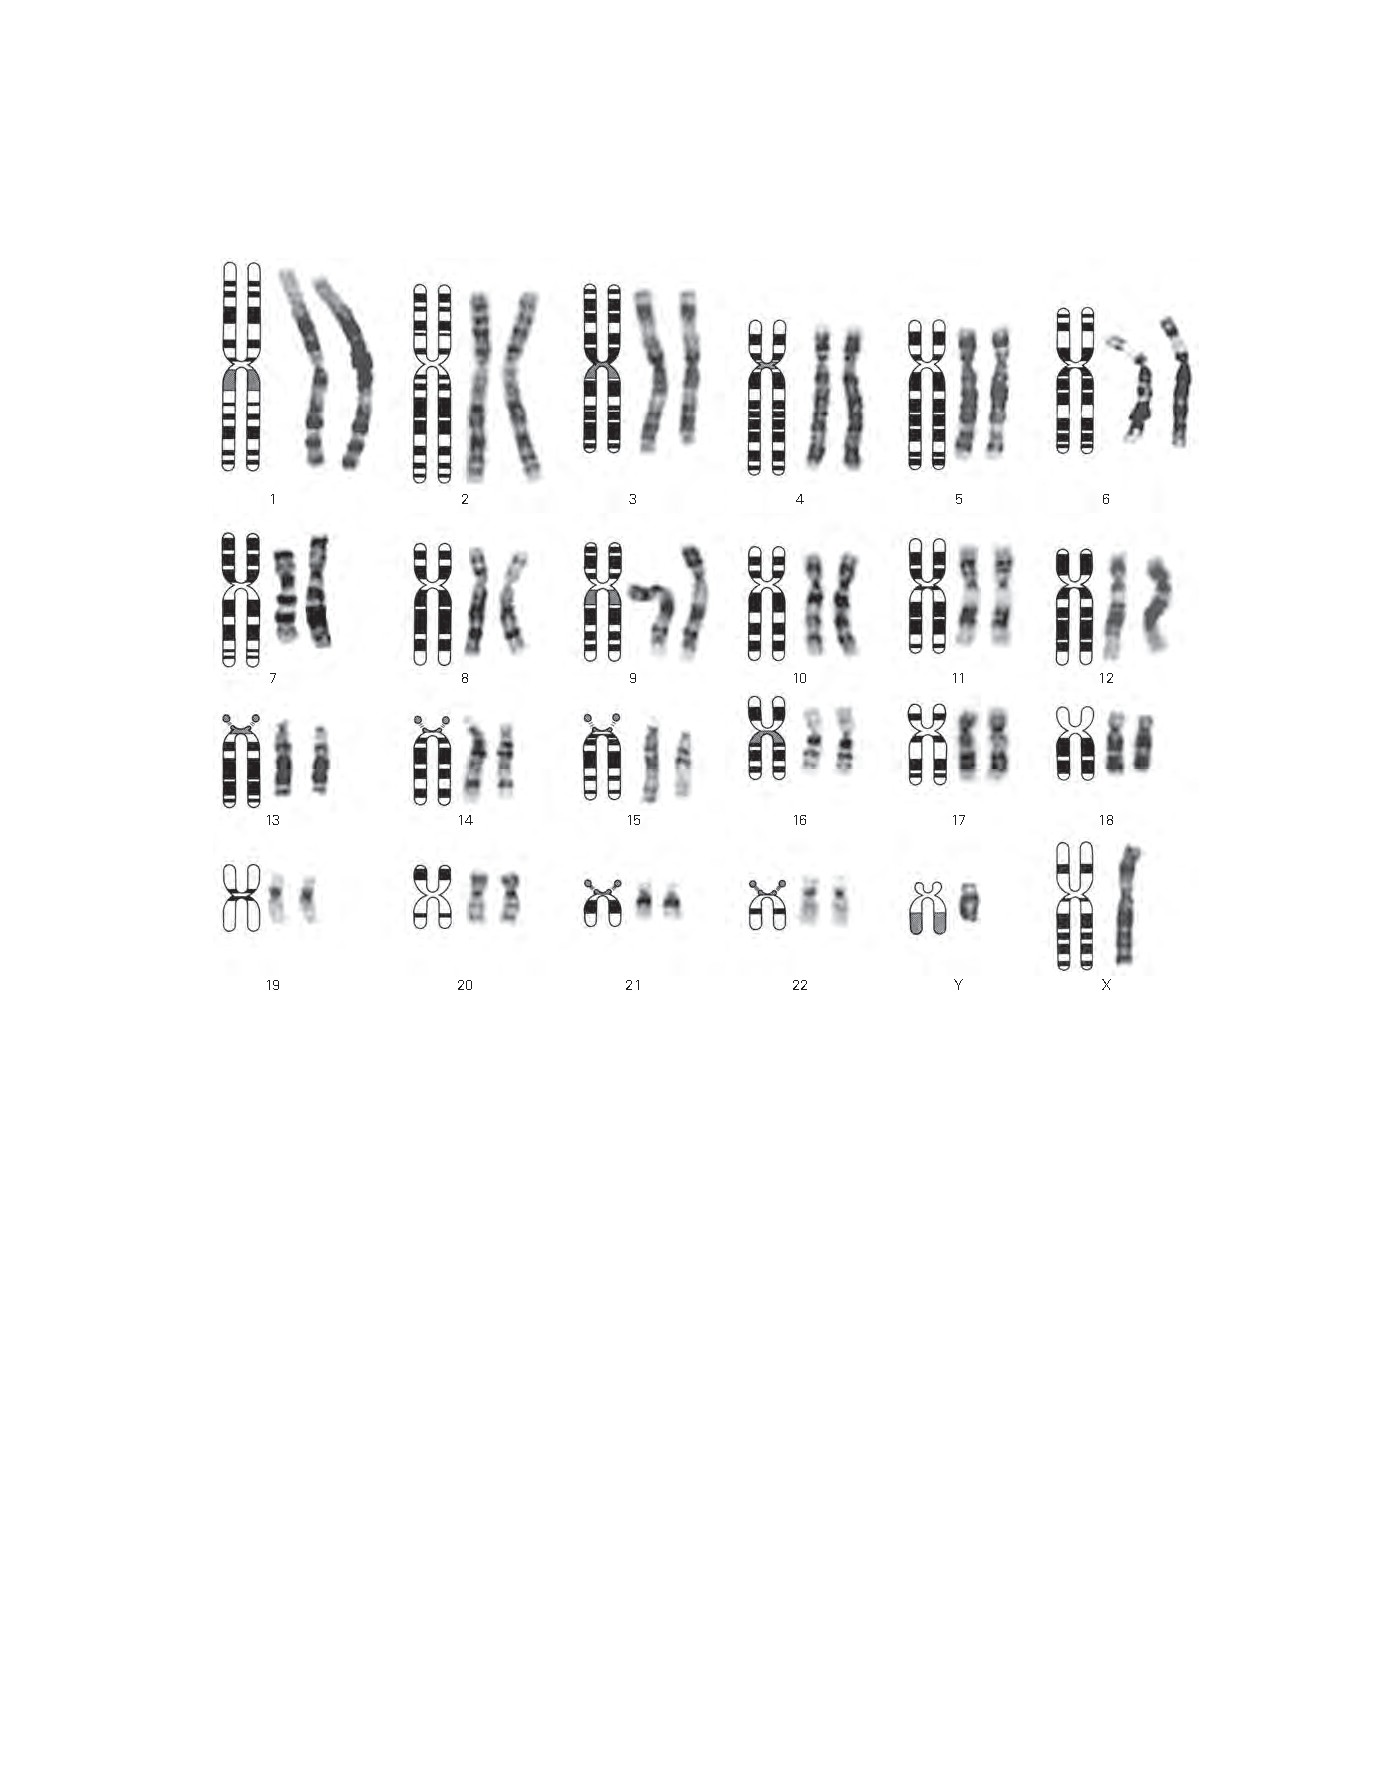
\includegraphics[width=0.8\linewidth]{chap02/fig_2_4}
	\caption{中期正常人类染色体的图解说明了每条染色体的独特形态。
		特征大小和特征亮区和暗区允许染色体彼此区分\cite{watoson1983recombinant}。}
	\label{fig:2_4}
\end{figure}


除了染色体上的基因外,极少数生物体基因通过线粒体传递,线粒体是执行代谢过程的细胞质细胞器。
所有儿童的线粒体都来自卵子,因此会从母亲传给孩子。
某些人类疾病,包括某些神经肌肉退行性疾病、某些形式的智力障碍和某些形式的耳聋,都是由线粒体\textit{脱氧核糖核酸}突变引起的。



\section{基因型和表现型之间的关系通常很复杂}

个体中特定常染色体基因的两个拷贝称为\textit{等位基因}。
如果两个\textit{等位基因}相同,则称个体在该位点是纯合的。
如果等位基因因突变而不同,则个体在该位点是杂合的。
男性是 X 染色体上基因的半合子。
一个群体可以有一个基因的大量等位基因;
例如,影响人眼颜色的单个\textit{2 型眼皮肤白化病}基因可以具有编码蓝色、绿色、淡褐色或棕色色调的等位基因。
由于这种变异,区分生物体的基因型(其基因组成)和表型(其外观)非常重要。
从广义上讲,基因型是构成个体基因组的整套等位基因;
狭义上,就是一个基因的特异等位基因。
相比之下,表型是对整个生物体的描述,是生物体基因型在特定环境中表达的结果。


如果突变表型仅在基因的两个等位基因都发生突变时才表达,则产生的表型称为隐性。
如果个体是突变等位基因的纯合子,或者如果他们在每个染色体上的给定基因中携带不同的破坏性等位基因(所谓的复合杂合子),就会发生这种情况。
隐性突变通常是由功能蛋白的丢失或减少引起的。
在人类和实验动物中普遍观察到突变性状的隐性遗传。


如果突变表型由一个突变体和一个野生型等位基因的组合产生,则表型特征和突变等位基因被认为是显性的。
一些突变是显性的,因为 50\% 的基因产物不足以形成正常表型(单倍体不足)。
其他显性突变导致异常蛋白质的产生或野生型基因产物在不适当的时间或地点的表达;
如果这对正常的蛋白质产物起拮抗作用,则称为显性失活突变。


当考虑具有同一基因的一个正常(野生型)等位基因和一个突变等位基因的后果时,基因型和表型之间的差异是显而易见的。
一系列神经发育障碍(包括孤独症和癫痫)的基因发现的最新进展表明,人类基因组对单倍体不足比以前认为的更敏感。
然而,虽然一个基因的两个拷贝的完全失活通常具有可靠的效果,但单倍体不足的严重性和表现在个体之间差异更大,这种现象称为可变、部分或不完全外显率。


干扰人类发育、细胞功能或行为的遗传变异落在共同等位基因(也称为多态性)和稀有变异之间的连续体上,前者通常对生物学和行为具有较小的个体影响,后者可能具有较大的生物学效应(方框~\ref{box:2_1})。
虽然这些分类是有用的概括,但在一些重要的案例中,常见的多态性会带来很大的疾病风险;
\textit{载脂蛋白E}基因的一种常见变异,存在于 16\% 的人口中,导致迟发性阿尔茨海默病的风险增加四倍。


\begin{proposition}[突变:遗传多样性的起源] \label{box:2_1}
	
	\quad \quad 尽管\textit{脱氧核糖核酸}复制通常是以高保真度进行的,但被称为突变的自发错误确实会发生。
	突变可能是由\textit{脱氧核糖核酸}中嘌呤和嘧啶碱基的损伤、\textit{脱氧核糖核酸}复制过程中的错误以及减数分裂过程中发生的重组引起的。
	
	
	\quad \quad 编码区内单个\textit{脱氧核糖核酸}碱基(也称为点突变)的变化分为五大类:
	
	
	1. 无声突变会改变碱基,但不会导致编码蛋白质发生明显变化。
	
	
	2. \textit{错义突变}是一种点突变,导致蛋白质中的一个氨基酸被另一个氨基酸取代;
	利用信息学和经验证据,这些突变被越来越多地分为至少两个亚类:损害蛋白质功能的突变和功能中性的突变。
	
	
	3. \textit{无义突变}是指其中指定特定氨基酸的编码区内的密码子(三重核苷酸)被终止密码子取代,导致蛋白质产物缩短(截短)。
	
	
	4. \textit{经典剪切位点突变}改变了指定外显子/内含子边界的核苷酸。
	
	5. \textit{框移突变}是指其中核苷酸的小片段插入或缺失改变了阅读框架,导致产生截短或异常的蛋白质。
	
	\quad \quad 在目前的文献中,属于后四类的突变(包括破坏性错义突变)通常被称为可能的基因破坏(LGD)突变。
	
	\quad \quad 在实验遗传学研究中,当生物体暴露于化学诱变剂或电离辐射时,突变的频率会大大增加。
	化学诱变剂倾向于诱导\textit{点突变},涉及单个\textit{脱氧核糖核酸}碱基对的变化或几个碱基对的缺失。
	电离辐射可诱导大量插入、缺失或易位。
	
	\quad \quad 在人类中,\textit{点突变}在\textit{卵母细胞}和精子中以较低的自发率发生,导致孩子出现突变,但父母双方都没有,称为\textit{新生突变}。
	每一代,整个基因组(约30亿个碱基对)都会发生70至90个单碱基变化,其中一个碱基对平均会导致蛋白质编码基因的\textit{错义突变}或\textit{无义突变}。
	父亲年龄较大的孩子新发点突变的数量增加,而母亲年龄较大的儿童染色体异常的频率增加。
	
	
	\quad \quad 随着2001年人类基因组测序和检测基因变异的高分辨率方法的不断提高,现在也很清楚,点突变并不是人类之间唯一的序列差异。
	某些序列可能在染色体上缺失或重复多次,因此在不同的个体中可能具有不同数量的拷贝。
	超过一个碱基和少于1000个碱基对的变化被称为\textit{插入缺失突变}。
	当这种变异包含超过1000个碱基对时,它们被称为\textit{拷贝数变异}。
	
	
	\quad \quad 任何基因变异对疾病或综合征的贡献都可以被称为简单的(或孟德尔的)或复杂的。
	一般来说,一个简单的或孟德尔突变是一个足以赋予表型而没有额外遗传风险的突变。
	这并不意味着每个有突变的人都会表现出完全相同的表型。
	然而,特定疾病等位基因和表型之间通常存在高度可靠的关系,这种关系接近一对一的关系(如镰状细胞性贫血或亨廷顿舞蹈症)。
	
	
	\quad \quad 相反,复杂的遗传疾病是指遗传风险因素改变了疾病的概率,但并不是完全的因果关系。
	这种遗传贡献可能涉及罕见的突变、常见的多态性或两者兼有,并且通常是非常异质的,多个不同的基因和等位基因具有增加风险或发挥保护作用的能力。
	大多数复杂的疾病也与环境有关。
	
		
\end{proposition}



\section{基因在进化中得以保存}

2001年报道了人类基因组近乎完整的核苷酸序列,许多动物基因组的完整核苷酸序列也已被破译。
这些基因组之间的比较得出了一个令人惊讶的结论:
独特的人类物种并非源于独特的新人类基因发明。


人类和黑猩猩在生物学和行为上有很大不同,但它们 99\% 的蛋白质编码基因是相同的。
此外,人类大约 2 万个基因中的大部分也存在于其他哺乳动物(例如小鼠)中,并且超过一半的人类基因与无脊椎动物(例如蠕虫和苍蝇)中的基因非常相似(图~\ref{fig:2_5})。
这一令人惊讶的发现得出的结论是,人类与其他动物共有的古老基因以新的方式受到调节,从而产生新的人类特性,例如产生复杂思想和语言的能力。


\begin{figure}[htbp]
	\centering
	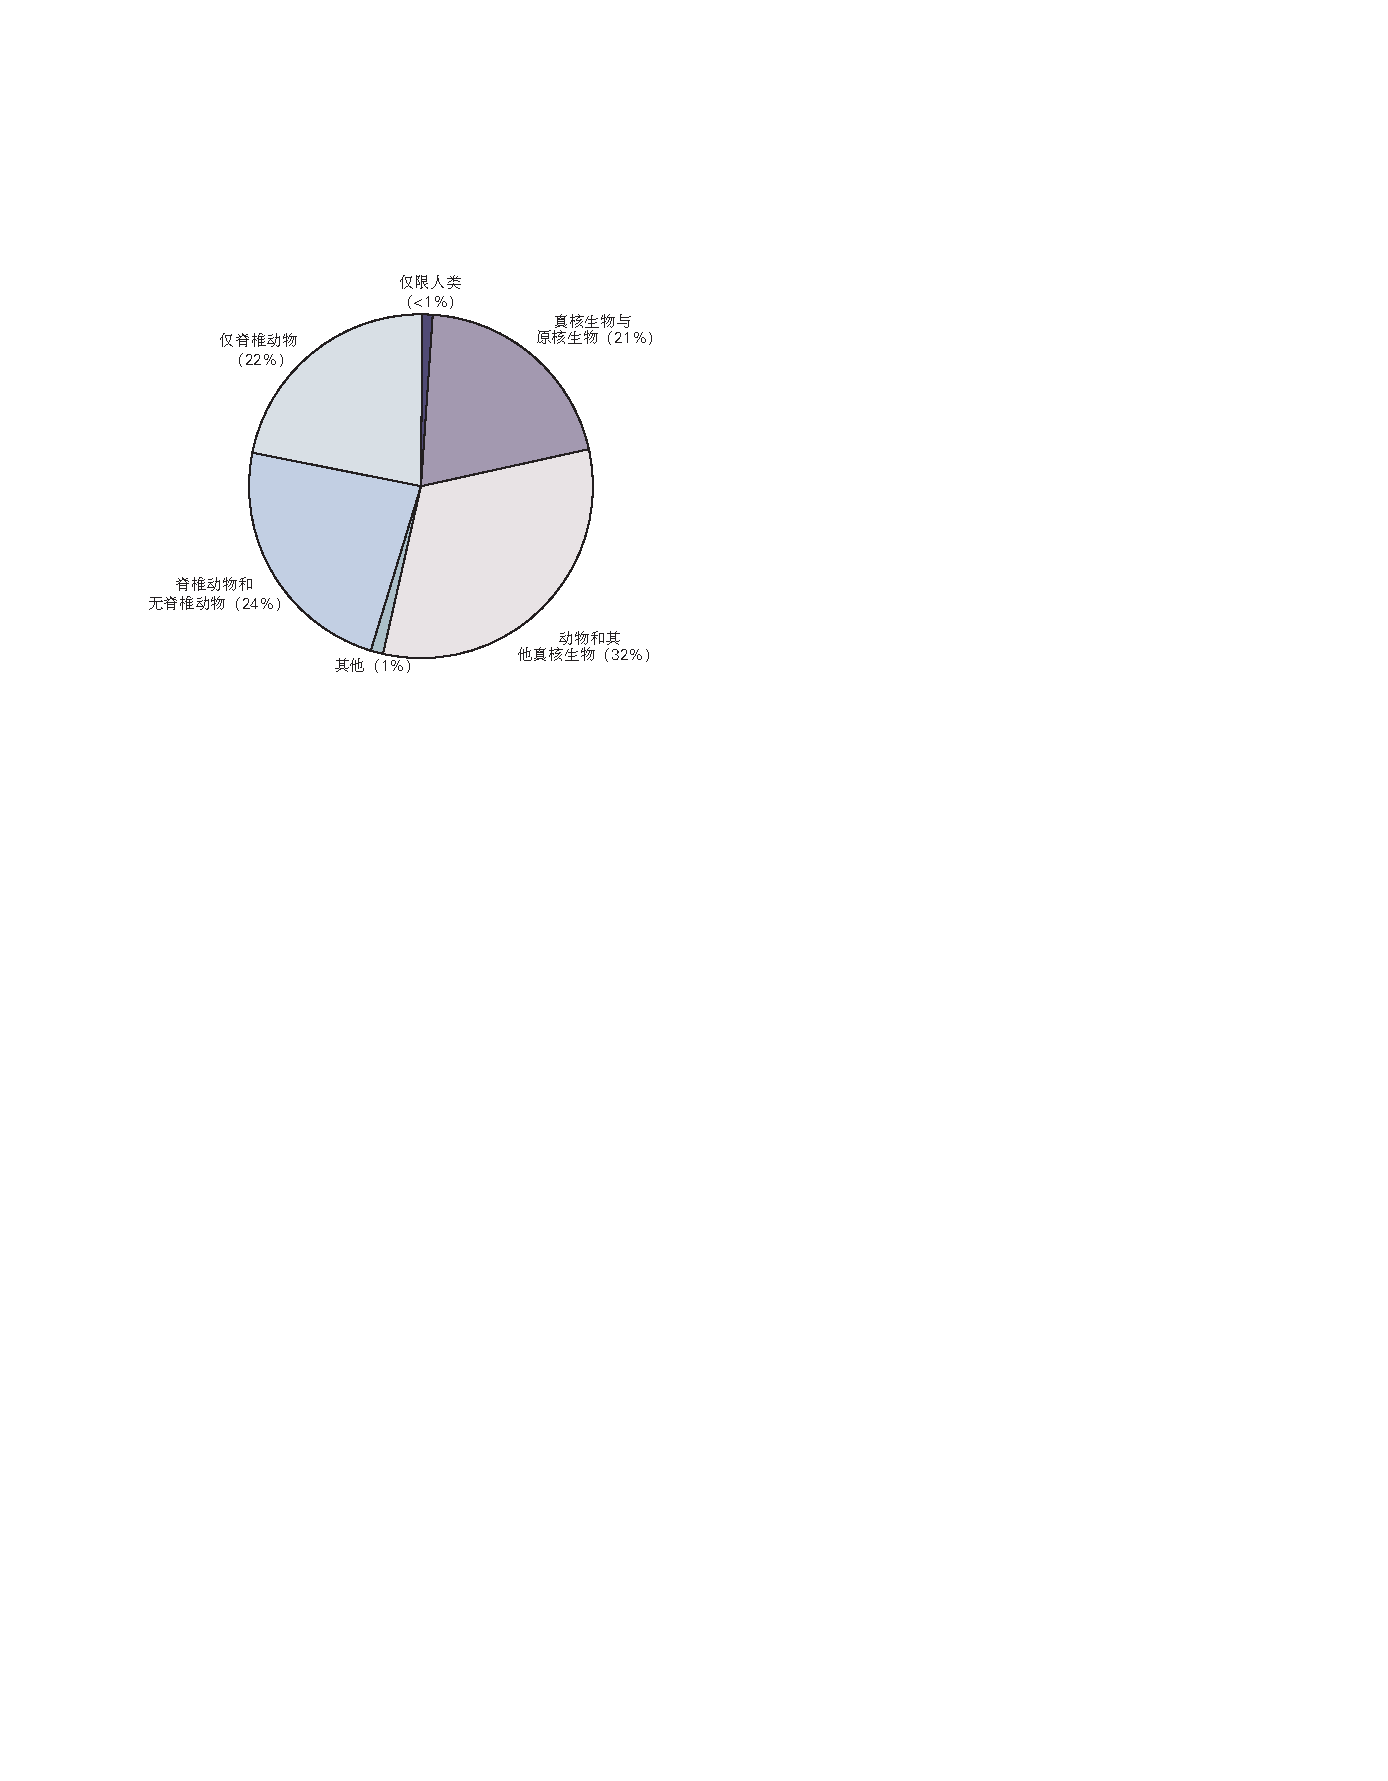
\includegraphics[width=0.5\linewidth]{chap02/fig_2_5}
	\caption{大多数人类基因都与其他物种的基因有关。
		不到 1\% 的人类基因是人类特有的;其他基因可能为所有生物、所有真核生物、仅动物或仅脊椎动物共享\cite{international2001initial}。}
	\label{fig:2_5}
\end{figure}


由于在整个进化过程中基因的这种保守性,对一种动物的研究的见解通常可以应用于具有相关基因的其他动物,这是一个重要的事实,因为动物实验通常是可能的,而人类实验却不可能。
例如,编码与人类基因相似的氨基酸序列的小鼠基因通常具有与直向同源人类基因相似的功能。


大约一半的人类基因具有已从其他生物体的直系同源基因中证明或推断出的功能(图~\ref{fig:2_6})。
人类、苍蝇甚至单细胞酵母共有的一组基因编码用于中间代谢的蛋白质;
\textit{脱氧核糖核酸}、\textit{核糖核酸}和蛋白质的合成;
细胞分裂; 和细胞骨架结构、蛋白质运输和分泌。


\begin{figure}[htbp]
	\centering
	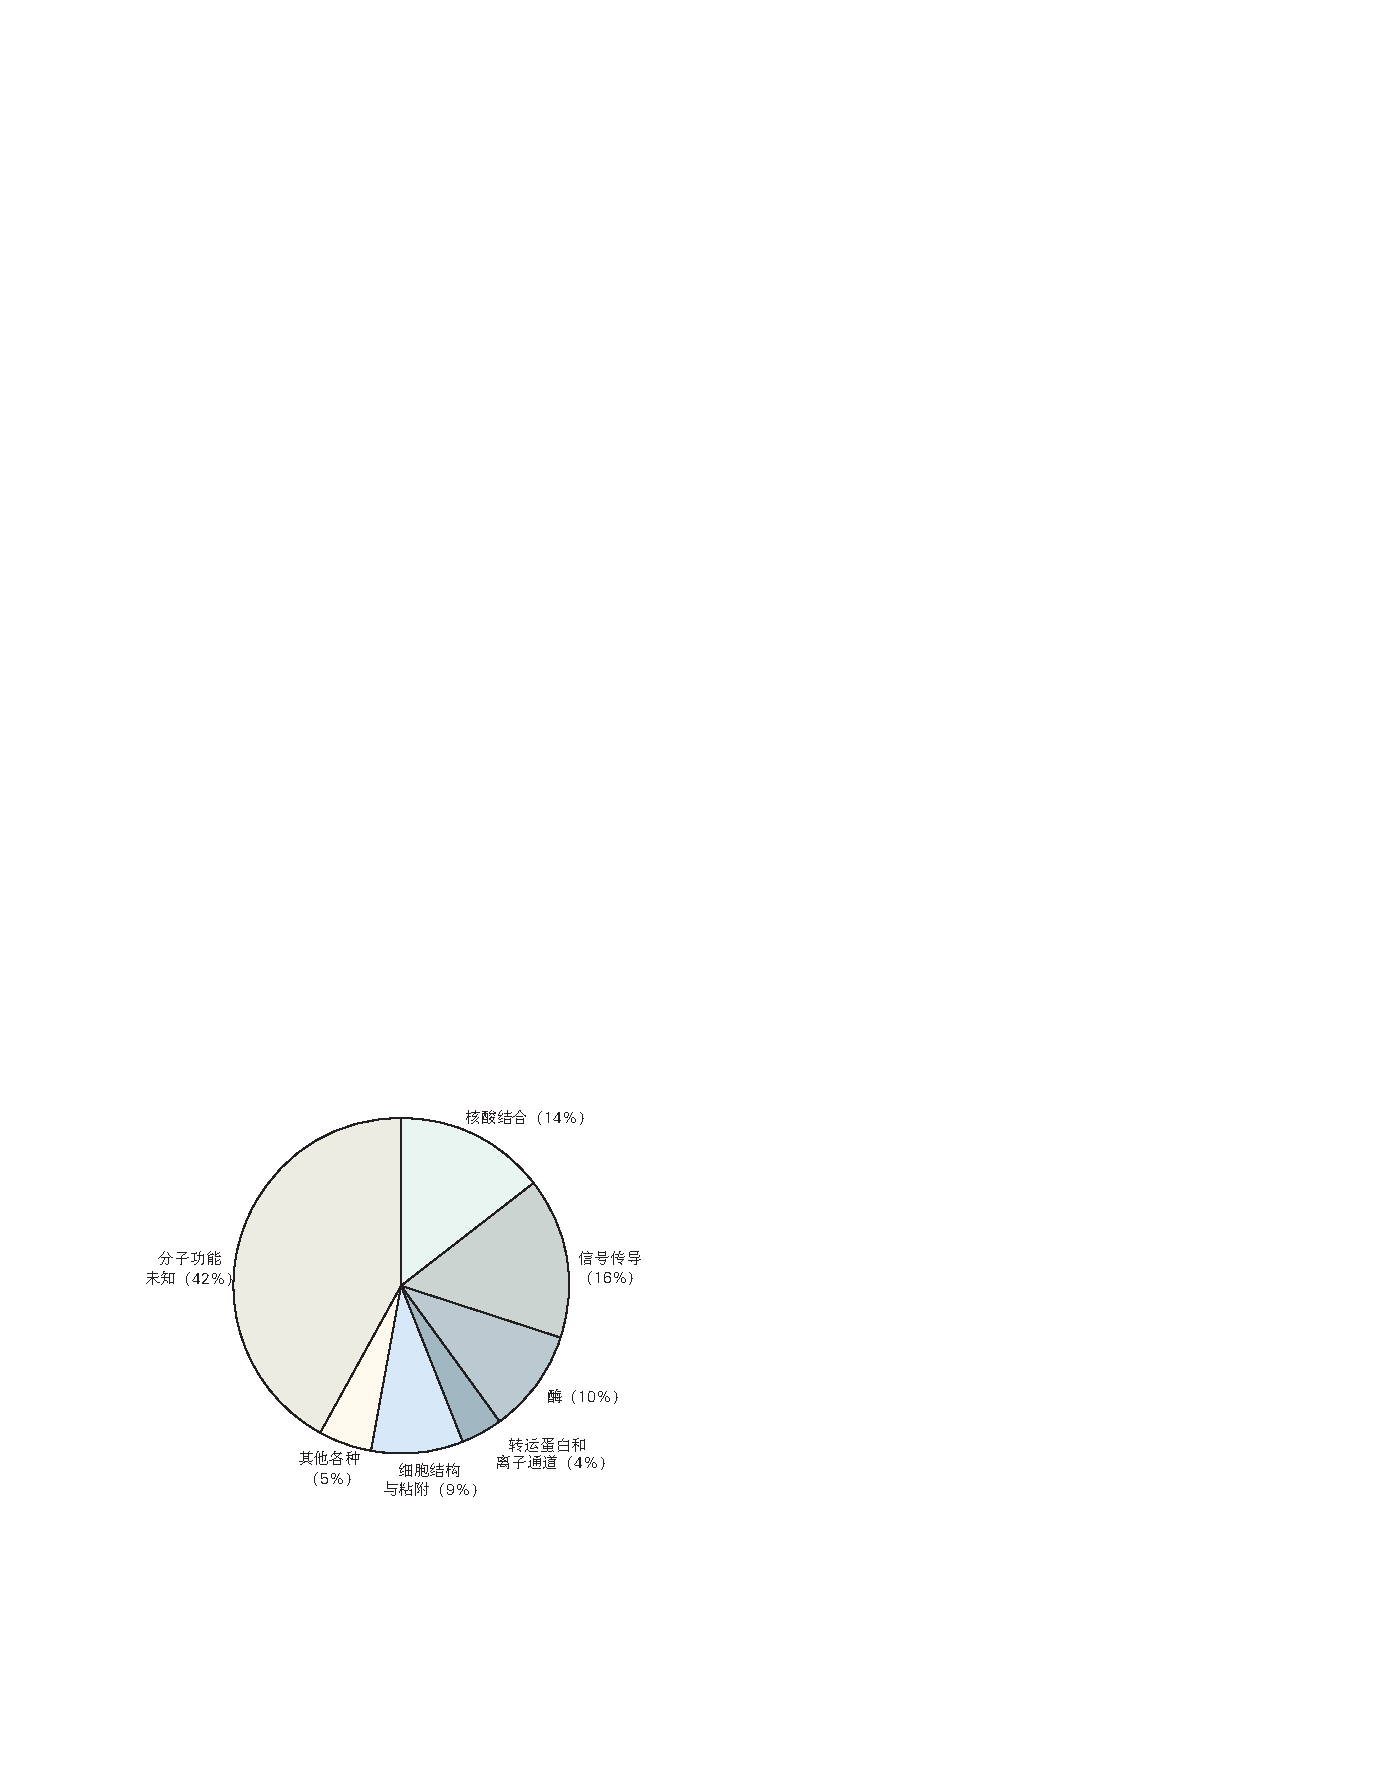
\includegraphics[width=0.5\linewidth]{chap02/fig_2_6}
	\caption{26,383 个人类基因的预测分子功能\cite{venter2001sequence}。}
	\label{fig:2_6}
\end{figure}


从单细胞生物到多细胞动物的进化伴随着与细胞间信号传导和基因调控有关的基因的扩展。
多细胞动物(例如蠕虫、苍蝇、小鼠和人类)的基因组通常编码数千个跨膜受体,比单细胞生物中存在的多得多。 
这些跨膜受体用于发育过程中的细胞间通讯、神经元之间的信号传递以及作为环境刺激的传感器。
多细胞动物的基因组还编码 1,000 种或更多不同的\textit{脱氧核糖核酸}结合蛋白,这些蛋白调节其他基因的表达。


人类的许多跨膜受体和\textit{脱氧核糖核酸}结合蛋白与其他脊椎动物和无脊椎动物的特定直系同源基因相关。
通过列举动物共有的遗传基因,我们可以推断出神经元发育、神经传递、电兴奋性和基因表达的基本分子通路存在于蠕虫、苍蝇、小鼠和人类的共同祖先中。
此外,对动物和人类基因的研究表明,人脑中最重要的基因是那些在整个动物系统发育过程中最保守的基因。
哺乳动物基因与其无脊椎动物基因之间的差异通常是由哺乳动物基因复制或基因表达和功能的细微变化引起的,而不是全新基因的产生。



\section{可以在动物模型中研究行为的遗传调控}

由于人类和动物基因之间的进化保守性,在动物模型中研究构成行为基础的基因、蛋白质和神经回路之间的关系可能会深入了解人类的这些关系。
在基因功能研究中应用了两个重要策略并取得了巨大成功。


在经典的遗传分析中,生物体首先受到化学诱变或辐射诱导随机突变,然后筛选影响感兴趣行为(例如睡眠)的可遗传变化。
这种方法不会对所涉及的基因类型施加偏见;
它是对所有可能导致可检测到的变化的突变的随机搜索。 
可遗传变化的遗传追踪允许识别突变生物体中改变的个体基因。
因此,经典遗传学的发现路径从表型到基因型,从生物体到基因。
在反向遗传学中,特定的感兴趣基因被作为改变的目标,产生转基因动物,并研究具有这些改变基因的动物。
这种策略既有重点又有偏见——一个是从特定基因开始——发现的途径从基因型到表型,从基因到生物体。


这两种实验策略及其更微妙的变化构成了实验遗传学的基础。
经典和反向遗传学的基因操作是在实验动物身上进行的,而不是在人类身上。



\subsection{转录振荡器调节苍蝇、小鼠和人类的昼夜节律}

Seymour Benzer 和他的同事在 1970 年左右发起了关于基因对行为影响的第一次大规模研究。
他们使用随机诱变和经典遗传分析来识别影响果蝇 Drosophila melanogaster 习得和先天行为的突变:昼夜节律(每天)节奏、求爱行为、运动、视觉感知和记忆(方框~\ref{box:2_2}~和方框~\ref{box:2_3})。
这些诱导突变对我们理解基因在行为中的作用产生了巨大影响。

\begin{proposition}[在实验动物中产生突变] \label{box:2_2}
	
	\quad \quad 苍蝇的随机诱变
	
	\quad \quad 果蝇(Drosophila)行为的遗传分析是在个体基因发生突变的果蝇身上进行的。
	突变可以通过化学诱变或插入诱变进行,这些策略可以影响基因组中的任何基因。
	类似的随机诱变策略被用于在线虫\textit{秀丽隐杆线虫}、斑马鱼和小鼠中产生突变。
	
	\quad \quad 化学诱变,例如用\textit{甲磺酸乙酯},通常会在基因中产生随机点突变。
	当被称为转座子的可移动\textit{脱氧核糖核酸}序列随机插入其他基因时,就会发生插入突变。
	
	\quad \quad 果蝇中最广泛使用的转座元件是P元件。
	P元素可以被修饰为携带眼睛颜色的遗传标记,这使得它们在遗传杂交中易于追踪,并且它们也可以被修饰以改变它们所插入的基因的表达。
	
	\quad \quad 为了引起P元素转位,携带P元素的果蝇菌株被杂交到不携带的果蝇菌株。
	这种遗传杂交会导致所产生的后代中P元素的不稳定和移位。
	P元素的动员导致其在随机基因中转移到新的位置。
	
	\quad \quad 小鼠的靶向诱变
	
	\quad \quad 哺乳动物基因分子操作的进展已经允许用突变版本精确替换已知的正常基因。
	产生突变小鼠菌株的过程涉及两种不同的操作。
	染色体上的基因被称为胚胎干细胞的特殊细胞系中的同源重组所取代,修饰后的细胞系被整合到胚胎的生殖细胞群中(图~\ref{fig:2_7}f)。
	
	\quad \quad 必须首先克隆感兴趣的基因。
	该基因发生突变,然后将选择性标记(通常是耐药性基因)引入突变片段中。
	然后将改变的基因引入胚胎干细胞,并分离出包含改变基因的细胞克隆。
	对每个克隆的\textit{脱氧核糖核酸}样本进行测试,以鉴定突变基因已整合到同源(正常)位点而不是其他一些随机位点的克隆。
	
	\quad \quad 当已经鉴定出合适的克隆时,在胚泡阶段(受精后3至4天)将细胞注射到小鼠胚胎中,此时胚胎由大约100个细胞组成。
	然后,这些胚胎被重新引入一只雌性体内,这只雌性已经为植入做了激素准备,并被允许足月。
	得到的胚胎是干细胞系和宿主胚胎之间的嵌合混合物。
	
	\quad \quad 小鼠的胚胎干细胞有能力参与发育的各个方面,包括生殖系。
	注射的细胞可以成为生殖细胞,并将改变后的基因传递给后代小鼠。
	这项技术已被用于在对神经系统发育或功能至关重要的各种基因中产生突变。
	
	\quad \quad 限制基因敲除和调控转基因表达
	
	\quad \quad 为了提高基因敲除技术的实用性,已经开发出将缺失限制在特定组织中或动物发育过程中特定点的细胞上的方法。
	区域限制的一种方法利用Cre/loxP系统。
	Cre/loxP系统是来源于P1噬菌体的位点特异性重组系统,其中噬菌体酶Cre重组酶催化34bp loxP识别序列之间的重组,这些序列通常不存在于动物基因组中。
	
	\quad \quad loxP序列可以通过同源重组插入胚胎干细胞的基因组中,使得它们位于感兴趣基因(称为floxed基因)的一个或多个外显子的侧翼。
	当干细胞被注射到胚胎中时,人们最终可以培育出一只小鼠,其中感兴趣的基因是游离的,并且仍然在动物的所有细胞中发挥作用。
	
	\quad \quad 然后可以产生第二批转基因小鼠,其在神经启动子序列的控制下表达Cre重组酶,该序列通常在受限的大脑区域中表达。
	通过将Cre转基因小鼠系与具有感兴趣的游离基因的小鼠系杂交,该基因将仅在表达Cre转基因的那些细胞中被删除。
	
	\quad \quad 在图2–8A所示的例子中,编码N-甲基天冬氨酸(NMDA)谷氨酸受体NR1(或GluN1)亚基的基因被loxP元件侧翼,然后在CaMKII启动子的控制下与表达Cre重组酶的小鼠系杂交,该启动子通常在前脑神经元中表达。
	在这个特定的细胞系中,表达偶然局限于海马CA1区,导致该脑区NR1亚基的选择性缺失(图~\ref{fig:2_8}B)。
	因为CaMKII启动子只在出生后激活基因转录,所以这种策略可以最大限度地减少早期发育变化。
	
	\quad \quad 除了基因表达的区域限制外,对基因表达时间的控制给研究者提供了额外的灵活性,并可以排除在成熟动物表型中观察到的任何异常是转基因产生的发育缺陷的结果的可能性。
	这可以在小鼠身上通过构建一种可以用药物开启或关闭的基因来实现。
	
	\quad \quad 一个是从创建两个小鼠行开始。
	品系1携带一种特殊的转基因,该转基因受启动子tetO的控制,而tetO通常只在细菌中发现。
	这个启动子本身不能启动基因;它需要被特定的转录调节因子激活。
	因此,第二组小鼠表达第二种转基因,该转基因编码一种杂交转录因子四环素反式激活因子(tTA),该因子识别并结合tetO启动子。
	tTA的表达可以置于小鼠基因组中的启动子的控制下,该启动子通常仅在特定类别的神经元或特定大脑区域中驱动基因转录。
	
	\quad \quad 当这两种小鼠交配时,一些后代将携带两种转基因。
	在这些小鼠中,tTA与tetO启动子结合并激活下游转基因。
	tTA转录因子之所以特别有用,是因为当它与某些抗生素(如四环素)结合时,它会失活,从而通过给小鼠服用抗生素来调节转基因表达。
	还可以产生表达被称为反向tTA(rtTA)的tTA突变形式的小鼠。
	这种反式激活剂不会与tetO结合,除非动物被喂食多西环素。
	在这种情况下,转基因总是被关闭,除非给药(图~\ref{fig:2_9})。
	
	\quad \quad \textit{核糖核酸}干扰和CRISPR改变基因功能
	
	\quad \quad 最后,可以通过现代分子工具靶向基因来灭活基因。
	一种这样的方法是\textit{核糖核酸}干扰,它利用了真核细胞中大多数双链RNA被常规破坏的事实;即使只有一部分是双链的,整个\textit{核糖核酸}也会被破坏。
	通过引入一个短\textit{核糖核酸}序列,人工地使选定的\textit{信使核糖核酸}变成双链,研究人员可以激活这一过程,降低特定基因的\textit{信使核糖核酸}水平。
	
\end{proposition}


\begin{figure}[htbp]
	\centering
	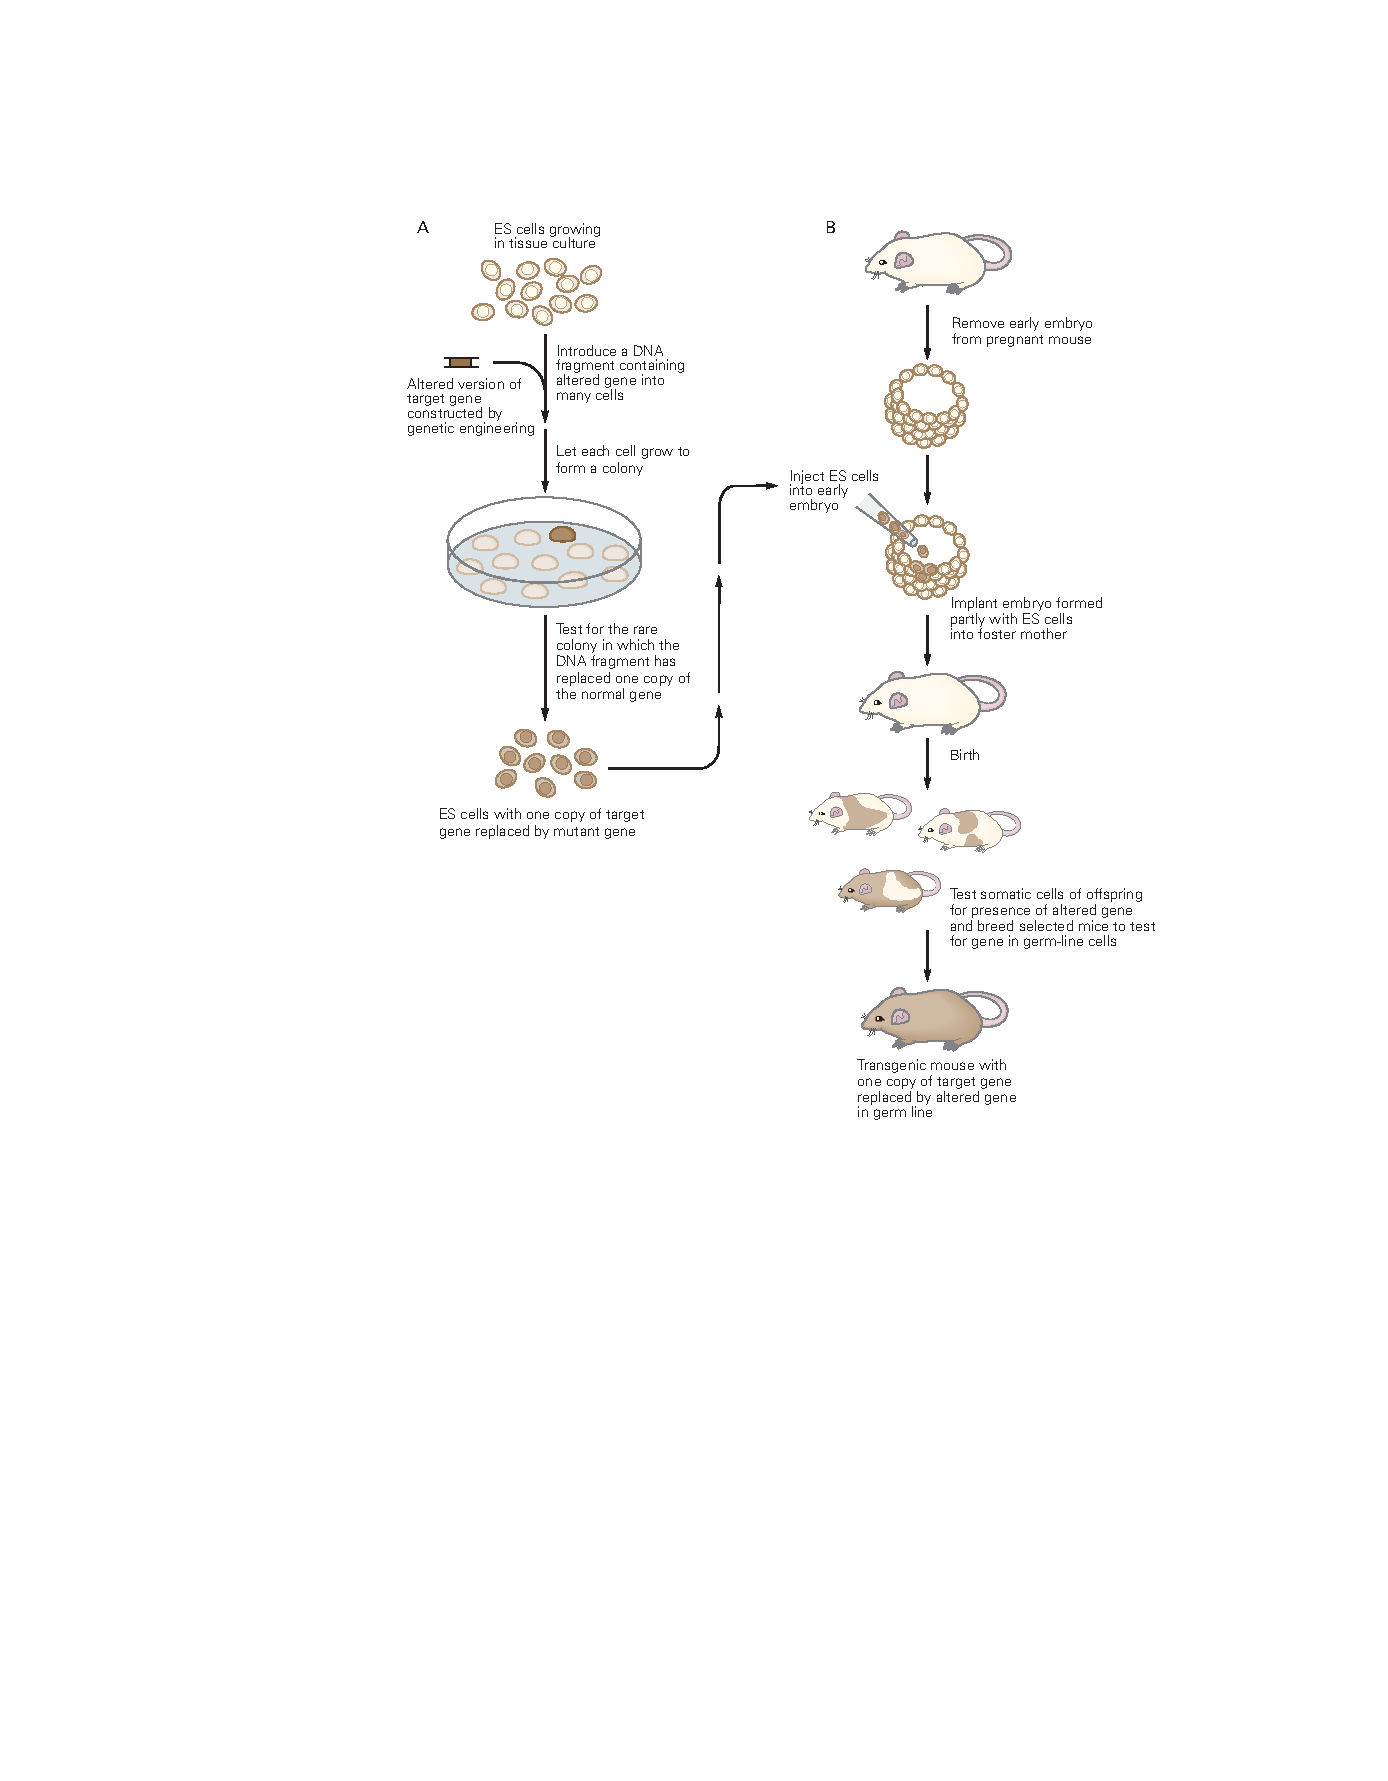
\includegraphics[width=0.5\linewidth]{chap02/fig_2_7}
	\caption{创造突变小鼠菌株\cite{alberts2017molecular}。
		\textbf{A.} 产生具有特定靶向突变的小鼠干细胞。
		\textbf{B.} 利用改变的胚胎干细胞创造转基因小鼠。}
	\label{fig:2_7}
\end{figure}


\begin{figure}[htbp]
	\centering
	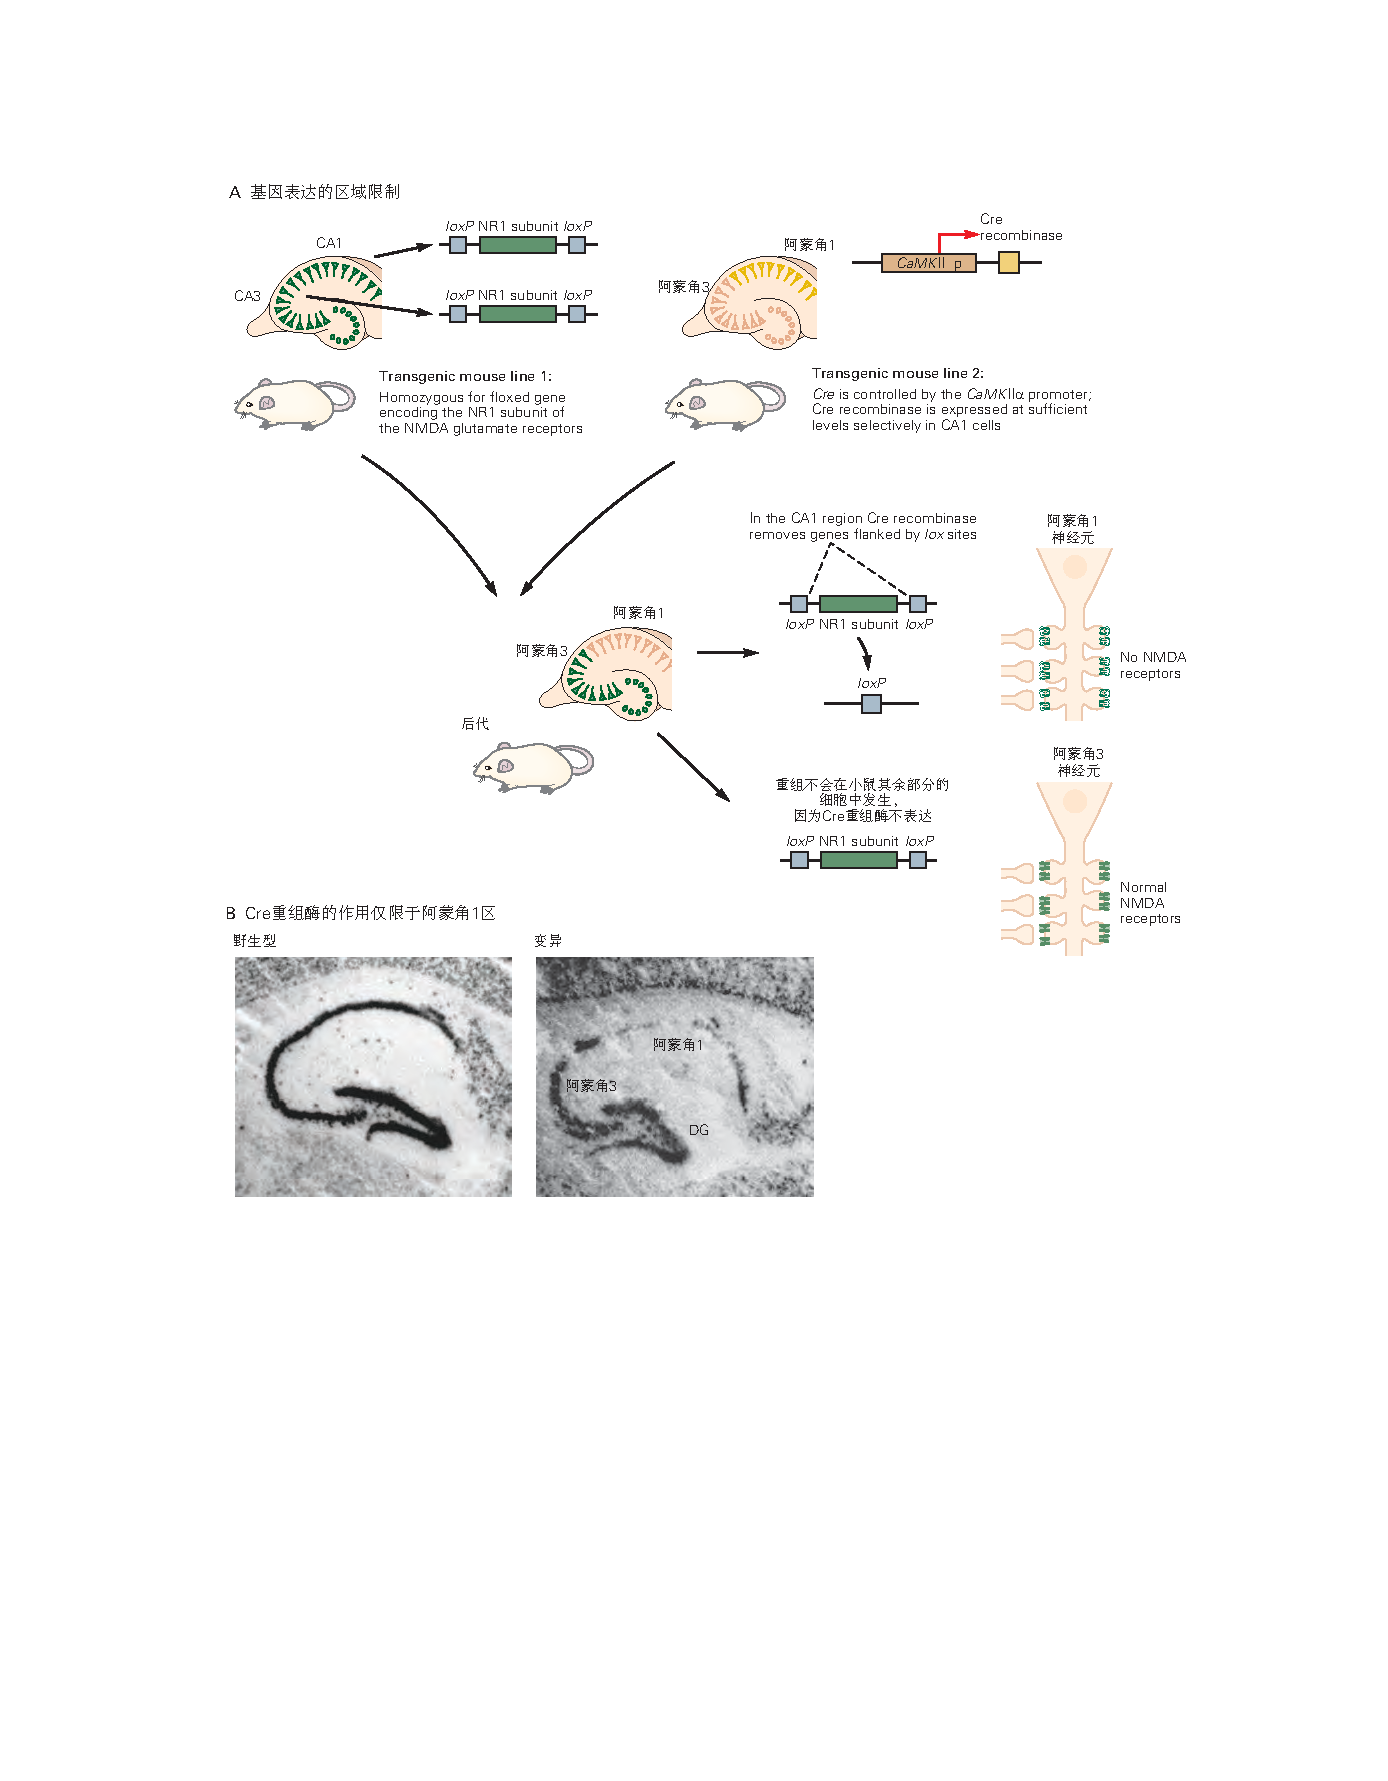
\includegraphics[width=0.5\linewidth]{chap02/fig_2_8}
	\caption{用于选择性区域基因敲除的Cre/loxP系统。
		\textbf{A.} 培育了一种小鼠系,其中编码NMDA受体NR1亚基的基因两侧有loxP遗传元件(转基因小鼠系1)。
		然后将这些所谓的“floxed NR1”小鼠与第二系小鼠杂交,其中编码Cre重组酶的转基因置于细胞类型或组织类型特异性转录启动子的控制下(转基因小鼠系2)。
		在本实施例中,来自CaMKIIa基因的启动子用于驱动Cre基因的表达。
		在携带Cre重组酶转基因的Floxy基因纯合的子代中,仅在驱动Cre表达的启动子活性的细胞类型中,通过Cre介导的loxP重组,Floxy的基因将被删除。
		\textbf{B.} 原位杂交用于检测野生型和突变小鼠海马切片中NR1亚基的\textit{信使核糖核酸},这些小鼠含有两个固定的NR1等位基因,并在CaMKIIa启动子的控制下表达Cre重组酶。
		在突变小鼠中,NR1的\textit{信使核糖核酸}表达(暗染色)在海马CA1区显著减少,但在CA3和齿状回(DG)保持正常\cite{tsien1996essential}。}
	\label{fig:2_8}
\end{figure}



\begin{proposition}[神经解剖学导航术语] \label{box:2_3}
	
	\quad \quad 转基因在苍蝇和老鼠中的引入
	
	\quad \quad 通过将\textit{脱氧核糖核酸}注射到新受精卵的细胞核中,可以在小鼠体内实验性地引入基因(图~\ref{fig:2_10})。
	在一些注射的卵子中,新基因或转基因被整合到其中一条染色体上的随机位点。
	由于胚胎处于单细胞阶段,整合的基因被复制并最终进入动物的所有(或几乎所有)细胞,包括种系。
	
	\quad \quad 通过将用于产生色素的基因注射到从白化病菌株获得的蛋中而拯救的外壳颜色标记基因来说明基因掺入。
	有色素斑块的小鼠表明\textit{脱氧核糖核酸}的成功表达。
	通过测试注射动物的\textit{脱氧核糖核酸}样本,证实了转基因的存在。
	
	\quad \quad 在苍蝇身上也使用了类似的方法。将待注射的\textit{脱氧核糖核酸}克隆到可转座元件(P元件)中。
	当注射到胚胎中时,\textit{脱氧核糖核酸}被插入生殖细胞核的\textit{脱氧核糖核酸}中。
	P元件可以被工程化以在特定时间和特定细胞中表达基因。
	转基因可以是恢复突变体功能的野生型基因,或者是改变其他基因表达或编码特异性改变的蛋白质的设计基因。
	
\end{proposition}


\begin{figure}[htbp]
	\centering
	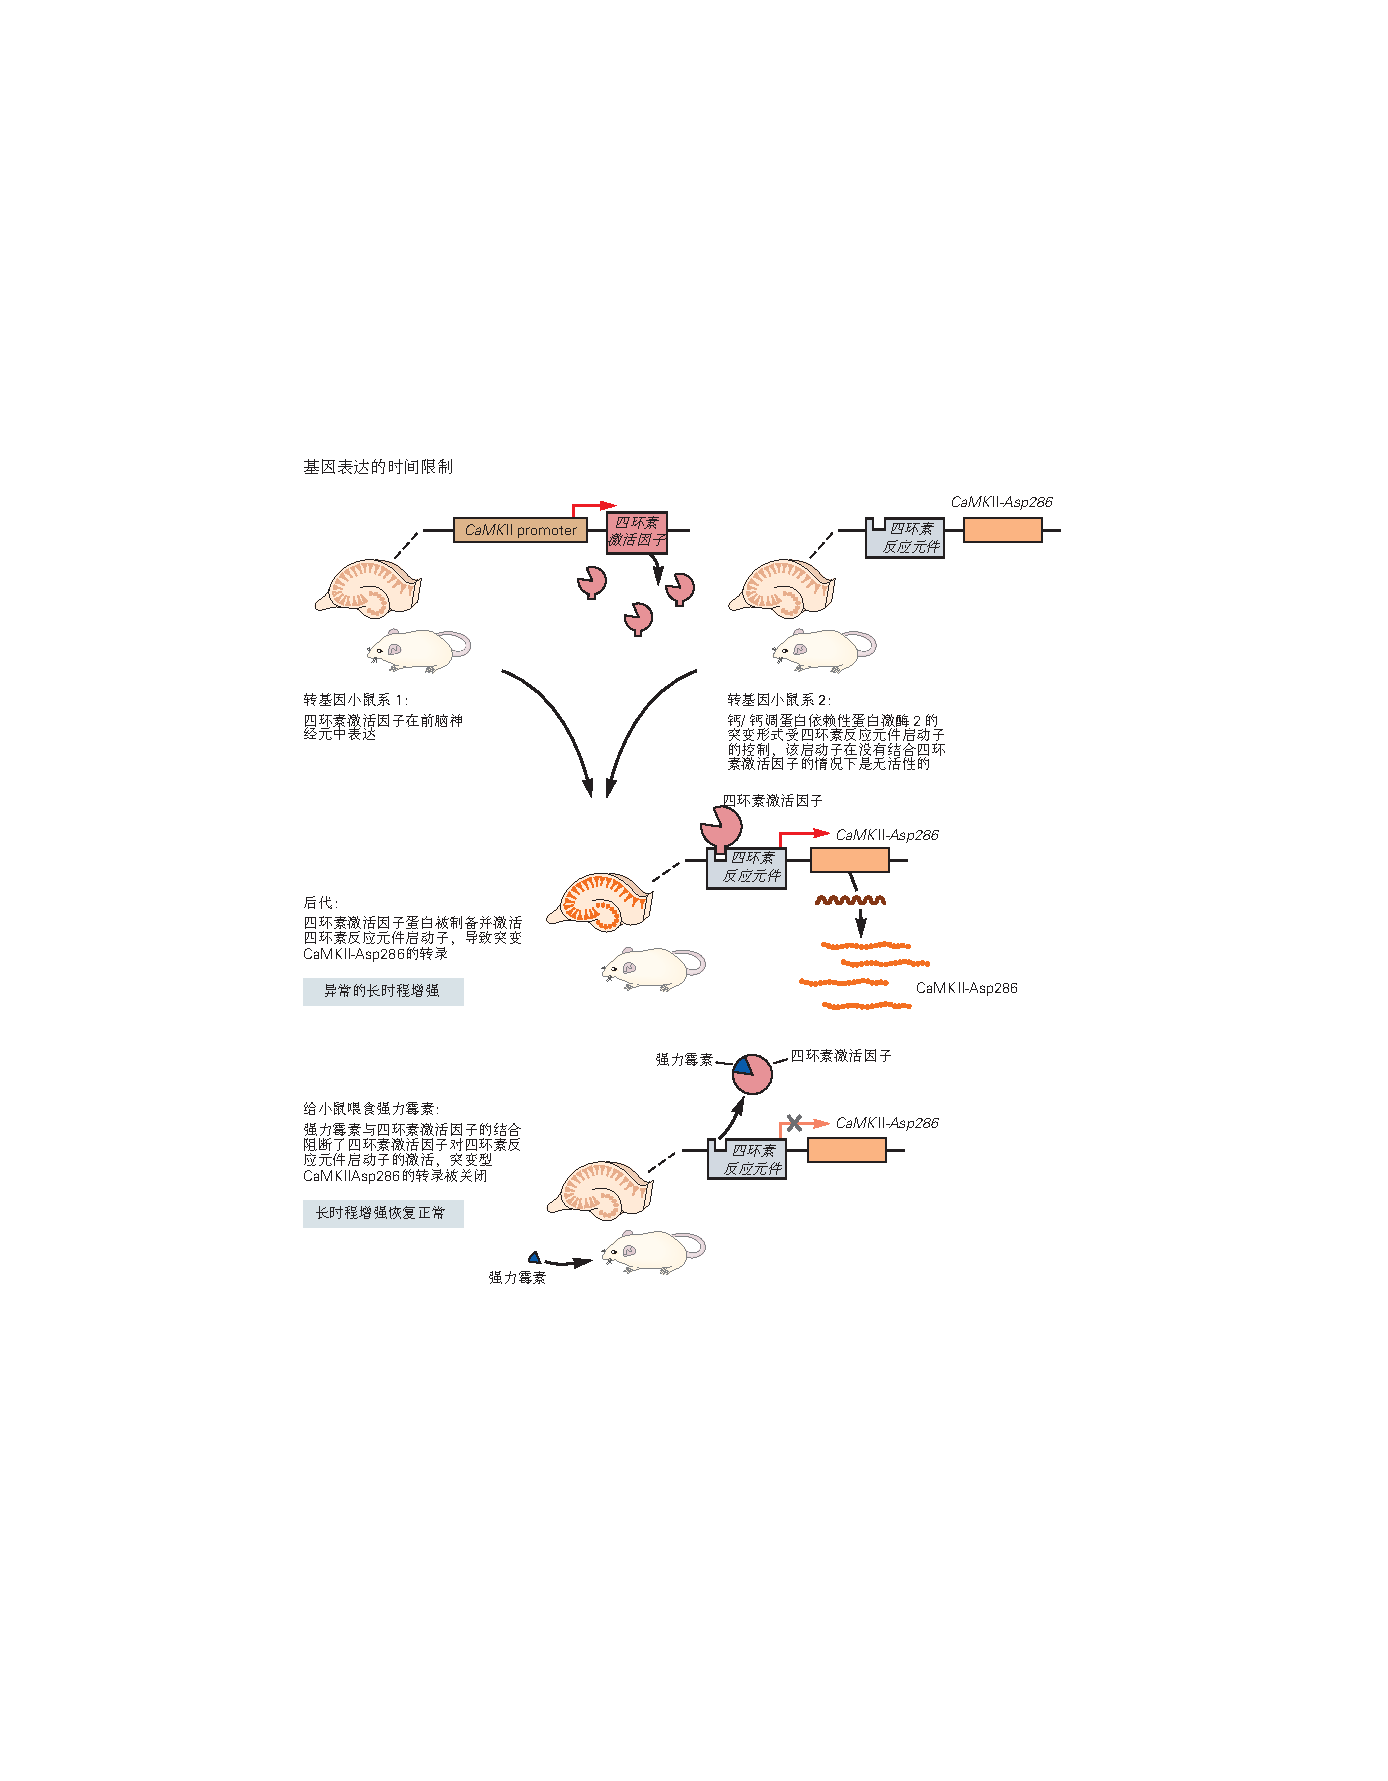
\includegraphics[width=0.5\linewidth]{chap02/fig_2_9}
	\caption{四环素系统用于转基因表达的时间和空间调控。培育了两个独立的转基因小鼠系。
		一个系在CaMKIIa启动子的控制下表达四环素反式激活子(tTA),这是一种结合了识别细菌tetO操纵子的细菌转录因子的工程蛋白。
		第二条线包含一个感兴趣的转基因——这里编码一种组成型活性形式的CaMKII(CaMKII–Asp286),它使激酶在没有 \ce{Ca^2+}的情况下持续活性——其表达受tetO的控制。
		当这两个系交配时,后代以仅限于前脑的模式表达tTA蛋白。
		当tTA蛋白与tetO结合时,它将激活感兴趣的下游基因的转录。
		给后代服用四环素(或多西环素)与tTA蛋白结合,并引起构象变化,导致该蛋白与tetO解除结合,阻断转基因表达。
		通过这种方式,小鼠将在前脑中表达CaMKII–Asp286,并且可以通过向小鼠施用多西环素来阻断这种表达\cite{mayford1996control}。}
	\label{fig:2_9}
\end{figure}


\begin{figure}[htbp]
	\centering
	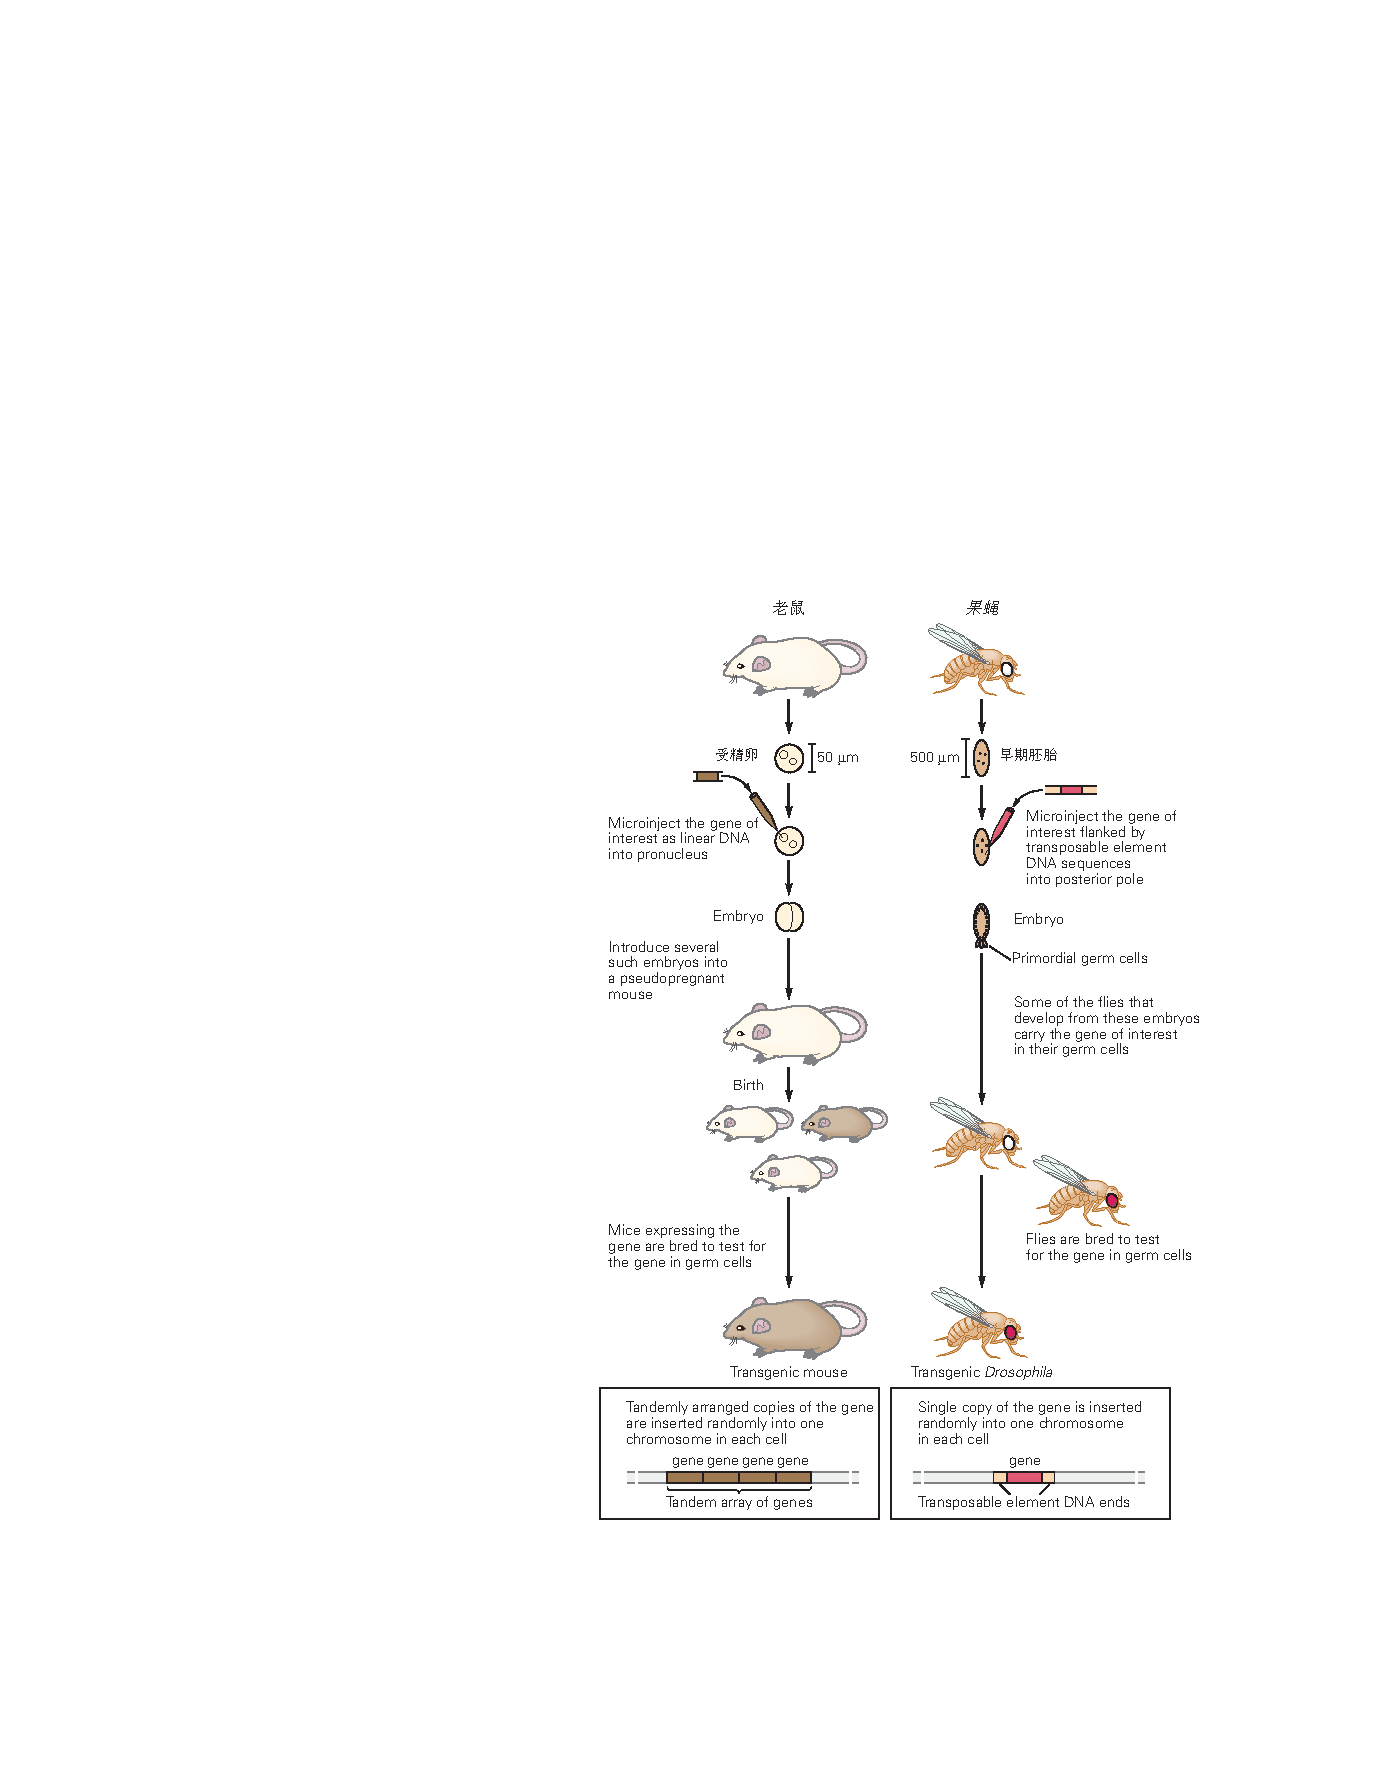
\includegraphics[width=0.6\linewidth]{chap02/fig_2_10}
	\caption{产生转基因小鼠和苍蝇。
		在这里,注射到小鼠体内的基因会导致毛色的变化,而注射到苍蝇体内的基因则会导致眼睛颜色的变化。
		在这两个物种的一些转基因动物中,\textit{脱氧核糖核酸}被插入不同细胞的不同染色体位点(见底部的插图)\cite{alberts2017molecular}。}
	\label{fig:2_10}
\end{figure}




我们对行为的昼夜节律控制的遗传基础有一个特别完整的了解。
动物的昼夜节律将某些行为与与太阳升起和落下相关的 24 小时周期联系起来。
昼夜节律调节的核心是一个在 24 小时周期内振荡的内在生物钟。
由于时钟的内在周期性,即使在没有光或其他环境影响的情况下,昼夜节律行为也会持续存在。


生物钟可以重新设置,这样昼夜循环的变化最终会导致内在振荡器发生匹配的变化,这是任何正在从时差反应中恢复过来的旅行者都熟悉的现象。
时钟由眼睛传输到大脑的光驱动信号重置。
最后,时钟驱动特定行为的效应通路,例如睡眠和运动。


Benzer 的团队搜索了数千只突变果蝇,以寻找由于指导昼夜节律振荡的基因发生突变而无法遵循昼夜节律的稀有果蝇。
从这项工作中,人们对生物钟的分子机制有了初步的了解。
周期或每个基因的突变影响果蝇内部时钟产生的所有昼夜节律行为。


有趣的是,每个突变都可以通过多种方式改变生物钟(图~\ref{fig:2_11})。
心律失常的 per 突变果蝇在任何行为中都没有表现出明显的内在节律,缺乏 per 基因的所有功能,因此 per 对节律行为至关重要。
维持基因某些功能的突变会导致节律异常。
长日等位基因产生 28 小时的行为周期,而短日等位基因产生 19 小时的行为周期。
因此 per 不仅是时钟的重要组成部分,它实际上是一个计时员,其活动可以改变时钟运行的速率。


\begin{figure}[htbp]
	\centering
	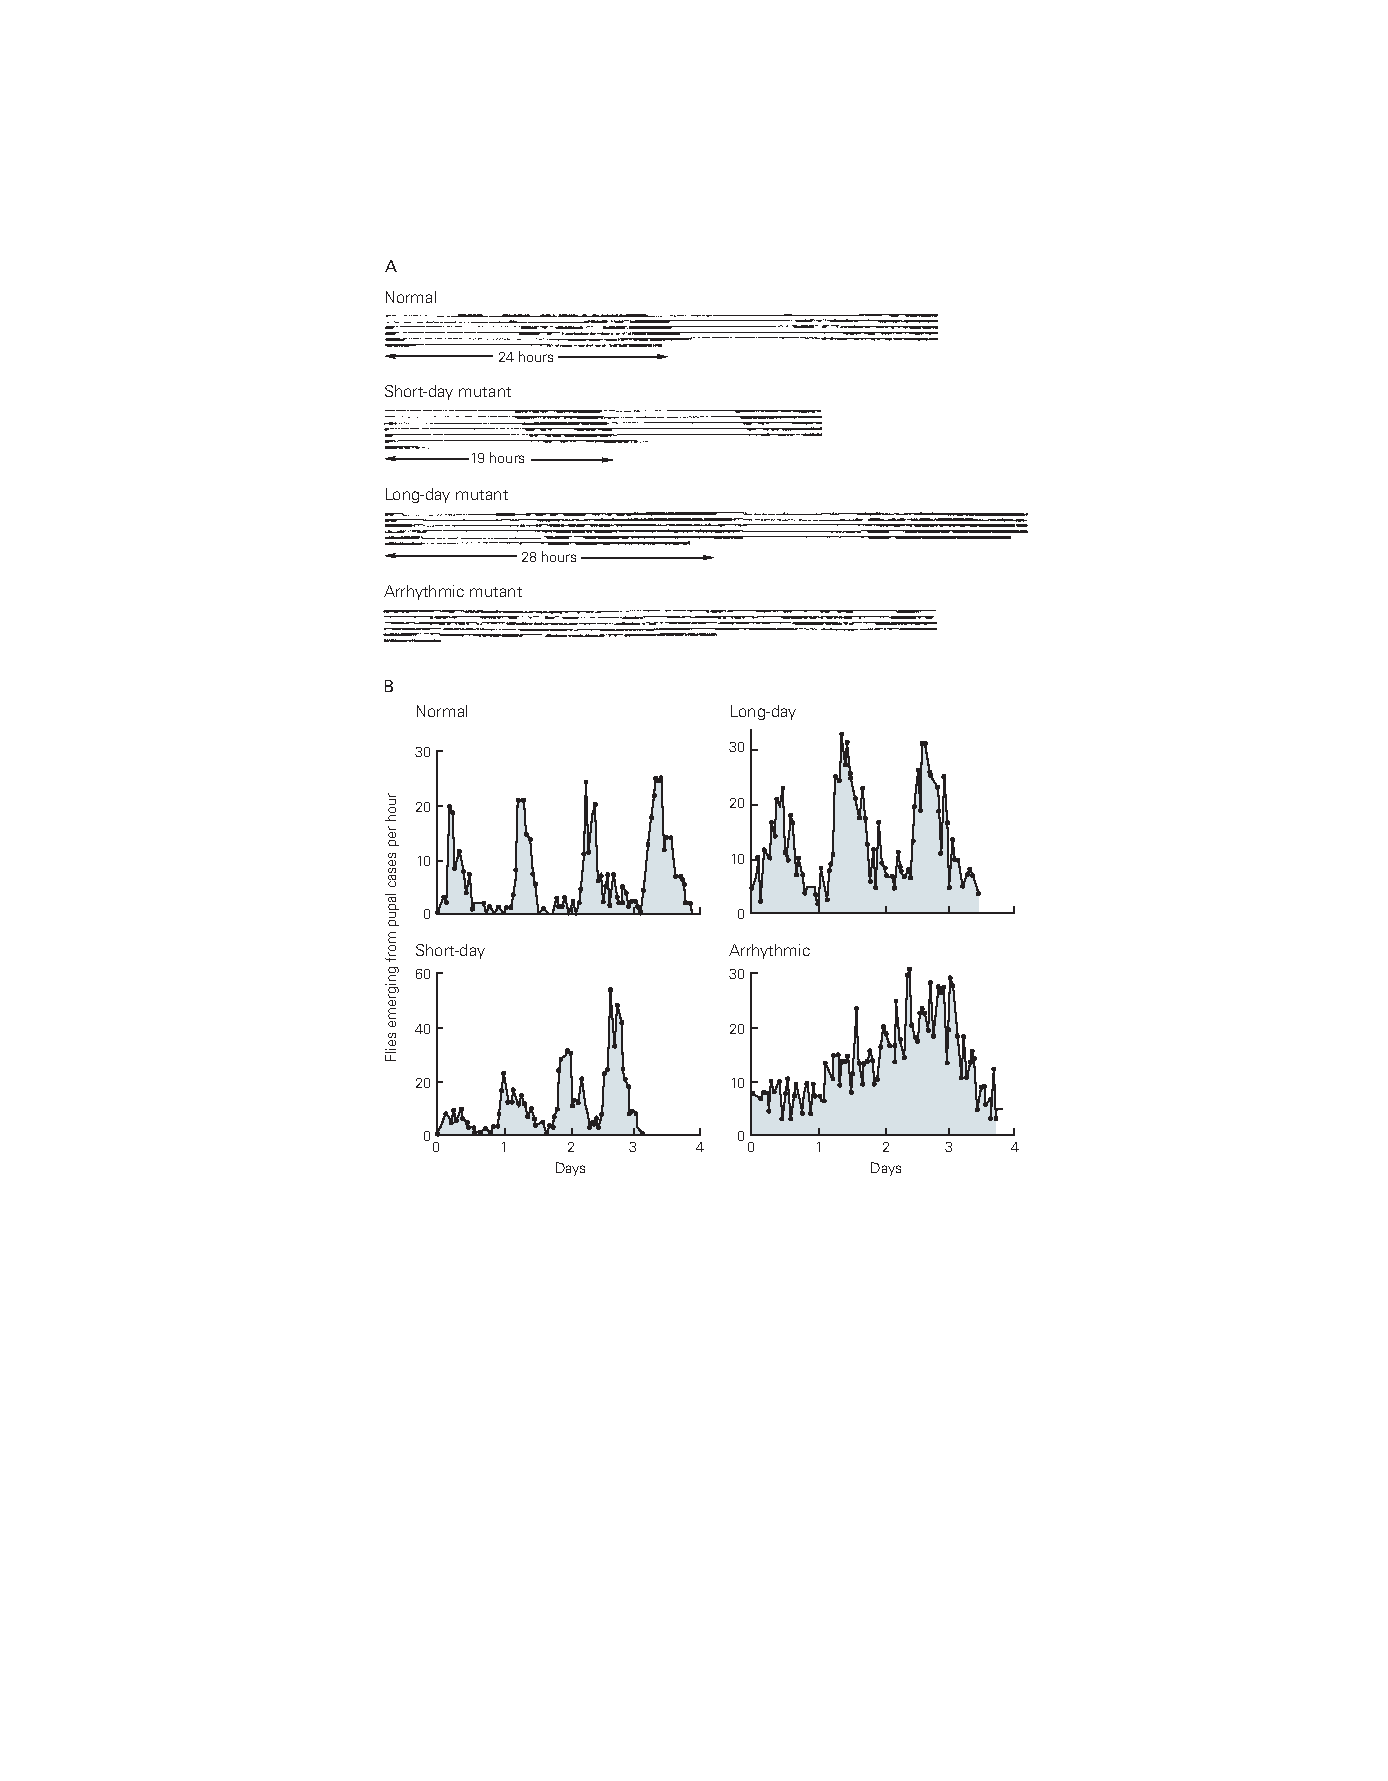
\includegraphics[width=0.5\linewidth]{chap02/fig_2_11}
	\caption{一个基因控制着果蝇行为的昼夜节律。
		周期或每个基因的突变会影响果蝇内部时钟调节的所有昼夜节律行为\cite{konopka1971clock}。
		\textbf{A.} 正常果蝇和 per 突变体的三种菌株的运动节律:短日照、长日照和心律失常。
		将苍蝇从 12 小时光照和 12 小时黑暗的循环转变为持续黑暗,然后在红外光下监测活动。
		记录中的粗段表示活动。
		\textbf{B.} 正常的成年苍蝇种群以周期性的方式从它们的蛹壳中出现,即使在持续的黑暗中也是如此。
		这些图显示了在持续黑暗的 4 天期间每小时出现的苍蝇数量(四个种群中的每一个)。
		出现没有任何可辨别的节律的心律失常突变种群。}
	\label{fig:2_11}
\end{figure}


per 突变体除了昼夜节律行为的改变外没有主要的不利影响。
这一观察很重要,因为在发现之前,许多人质疑是否可能存在动物生理需要不需要的真正“行为基因”。
Per 似乎确实是这样一种“行为基因”。


per 是如何保持时间的?
蛋白质产物 PER 是一种转录调节因子,可影响其他基因的表达。
PER 的水平全天受到监管。
清晨,PER 及其\textit{信使核糖核酸}较低。
在一天中,PER\textit{信使核糖核酸}和蛋白质积累,在黄昏后和夜间达到峰值水平。
然后水平下降,在下一个黎明前下降。
这些观察为昼夜节律之谜提供了答案——一个中央调节器在一天中出现和消失。
但它们也不令人满意,因为它们只是将问题往后推了一步——什么是 PER 循环?
这个问题的答案需要发现额外的时钟基因,这些基因在果蝇和老鼠身上都有发现。


受到果蝇昼夜节律筛查成功的鼓舞,约瑟夫·高桥 (Joseph Takahashi) 在 1990 年代开始在老鼠身上进行类似但劳动密集型得多的基因筛查。
他筛选了数百只突变小鼠,寻找昼夜运动周期发生改变的罕见个体,并发现了一个他称之为时钟的基因突变。
当时钟突变的纯合小鼠被转移到黑暗中时,它们最初会经历极长的昼夜节律周期,然后完全失去昼夜节律(图~\ref{fig:2_12})。
因此,时钟基因似乎可以调节昼夜节律的两个基本特性:昼夜节律周期的长度和在没有感觉输入的情况下节律性的持久性。
这些特性在概念上与果蝇中 per 基因的特性相同。


\begin{figure}[htbp]
	\centering
	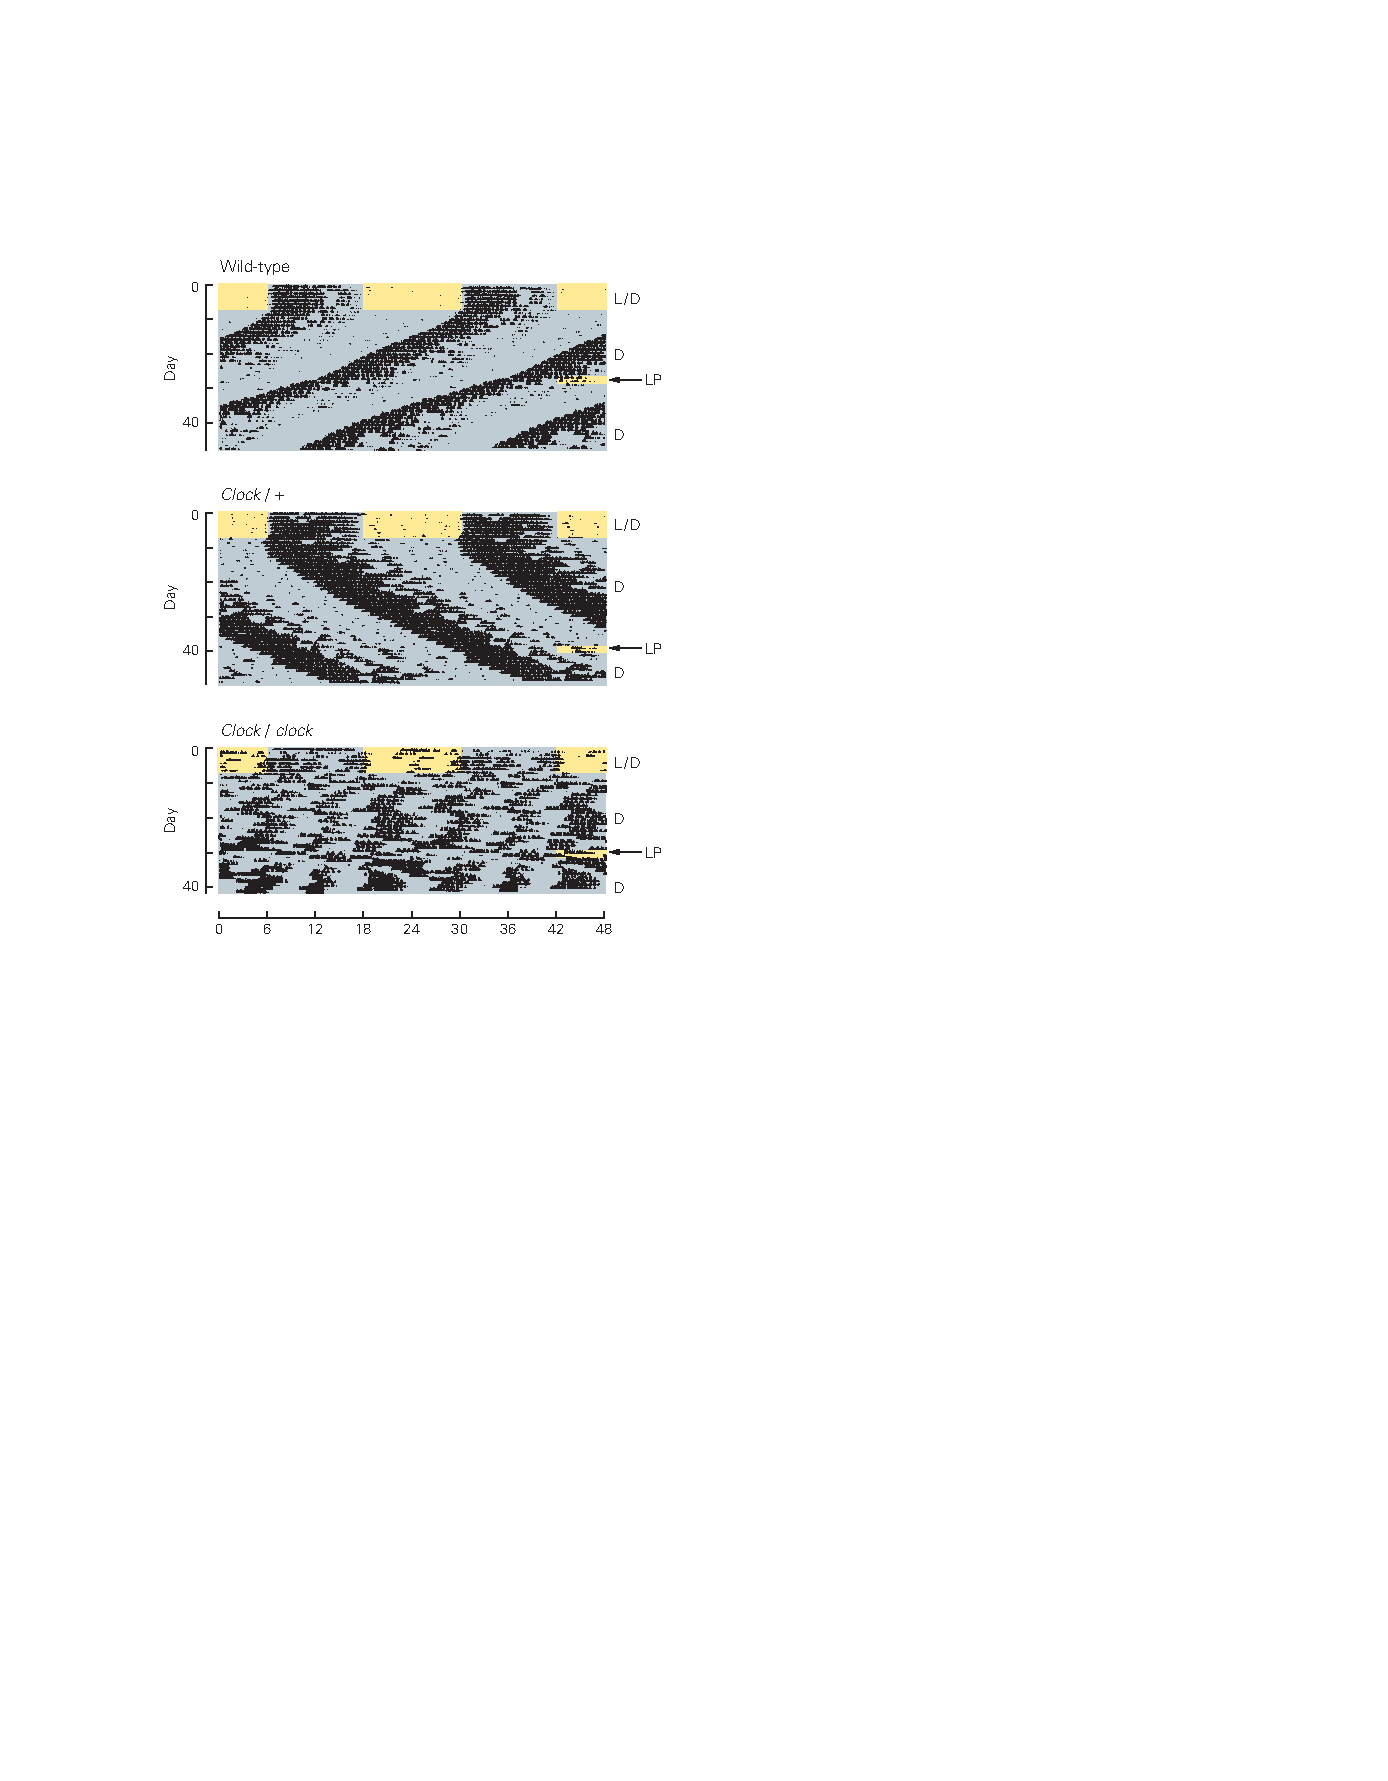
\includegraphics[width=0.5\linewidth]{chap02/fig_2_12}
	\caption{时钟基因对小鼠昼夜节律的调节。
		记录显示了三种动物的运动活动期:野生型、杂合型和纯合型。
		所有动物在前7天保持12小时的明暗(L/D)循环,然后转移到恒定黑暗(D)。
		之后,他们被暴露在6小时的光照期(LP)中以重置节奏。
		野生型小鼠的昼夜节律具有23.1小时的周期。
		杂合时钟/+小鼠的周期为24.9小时。
		纯合子时钟/时钟小鼠在转移到恒定黑暗时经历昼夜节律性的完全丧失,并在光照期后短暂表达28.4小时的节律\cite{takahashi1994forward}。}
	\label{fig:2_12}
\end{figure}


小鼠时钟基因与果蝇中的 per 基因一样,编码一个转录调节器,其活动在一天中波动。
小鼠 CLOCK 和果蝇 PER 蛋白也共享一个称为 PAS 结构域的结构域,这是转录调节因子子集的特征。
这一观察表明,相同的分子机制——PAS 结构域转录调节的振荡——控制着果蝇和小鼠的昼夜节律。


更重要的是,对果蝇和小鼠的平行研究表明,相似的转录调节因子组会影响这两种动物的生物钟。
在克隆小鼠时钟基因后,克隆了一个果蝇昼夜节律基因,发现它与小鼠时钟的关系比 per。
在另一项研究中,一种与 fly per 相似的小鼠基因被鉴定并通过反向遗传学灭活。
突变小鼠有昼夜节律缺陷,就像每个突变体都会飞一样。 
换句话说,果蝇和小鼠都使用时钟和每个基因来控制它们的昼夜节律。
一组基因,而不是一个基因,是生物钟的保守调节剂。


这些基因的表征导致了对昼夜节律分子机制的理解,并戏剧性地证明了这些机制在果蝇和小鼠中的相似性。
在果蝇和小鼠中,CLOCK 蛋白都是一种转录激活因子。 
它与伴侣蛋白一起控制决定运动活动水平等行为的基因的转录。
CLOCK 及其伙伴还刺激 per 基因的转录。
然而,PER 蛋白抑制 CLOCK 刺激每个基因表达的能力,因此随着 PER 蛋白的积累,每个转录下降(图~\ref{fig:2_13})。
24 小时周期的出现是因为 PER 蛋白的积累和激活在 per 转录后延迟了许多小时,这是 PER 磷酸化、PER 不稳定性以及与其他循环蛋白相互作用的结果。


\begin{figure}[htbp]
	\centering
	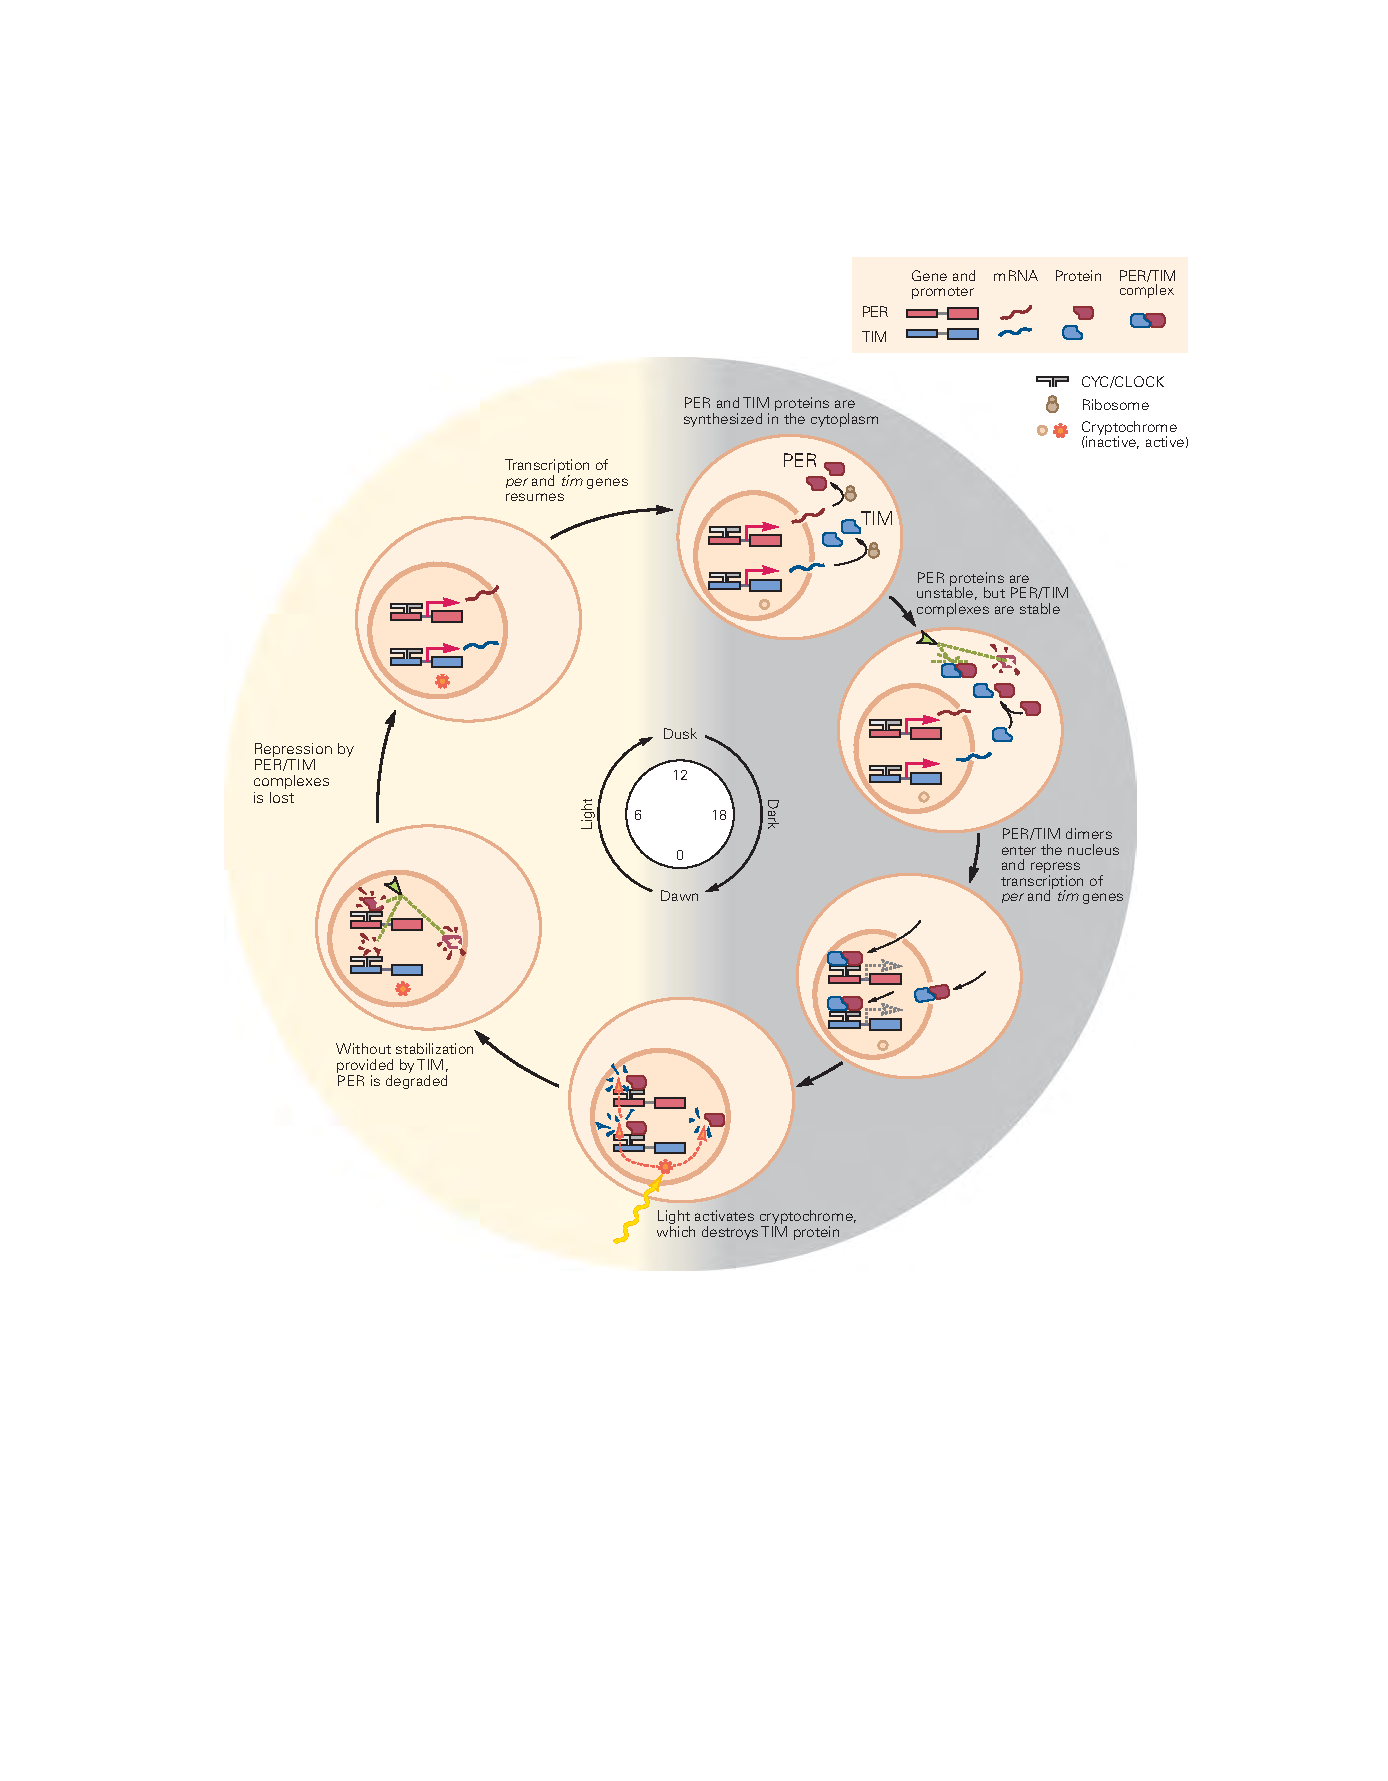
\includegraphics[width=0.5\linewidth]{chap02/fig_2_13}
	\caption{驱动昼夜节律的分子事件。
		控制生物钟的基因受两种核蛋白 PER 和 TIM 的调节。
		这些蛋白质慢慢积累,然后相互结合形成二聚体。
		一旦它们形成二聚体,它们就会进入细胞核并关闭包括它们自己在内的昼夜节律基因的表达。
		它们通过抑制刺激 per 和 tim 基因转录的 CLOCK 和 CYCLE 来实现。
		PER 蛋白非常不稳定; 其中大部分降解得如此之快,以至于它永远没有机会抑制每个转录的时钟依赖性。 
		PER 的降解受不同蛋白激酶的至少两种不同磷酸化事件的调节。
		当 PER 与 TIM 结合时,PER 受到保护免于降解。 
		随着 CLOCK 驱动越来越多的 per 和 tim 表达,足够的 PER 和 TIM 最终积累到两者可以结合并稳定彼此,此时它们进入细胞核,在那里它们自身的转录受到抑制。
		结果,per 和 tim 的\textit{信使核糖核酸}水平下降; 此后,PER 和 TIM 蛋白水平下降,CLOCK 可以(再次)驱动 per 和 tim \textit{信使核糖核酸}的表达。
		在白天,TIM 蛋白被光调节的信号通路(包括隐花色素)降解,因此 PER/TIM 复合物仅在夜间形成。
		CLOCK 蛋白诱导 PER 和 TIM 表达,但被 PER 和 TIM 蛋白抑制。}
	\label{fig:2_13}
\end{figure}


per、clock 和相关基因的分子特性产生了昼夜节律所必需的所有特性。

1. 昼夜节律基因转录随24小时周期变化:夜间PER活性高; CLOCK 白天活跃度很高。


2. 昼夜节律基因是相互影响\textit{信使核糖核酸}水平的转录因子,产生振荡。
CLOCK 按转录激活,PER 抑制 CLOCK 功能。


3. 昼夜节律基因还控制其他基因的转录,进而影响许多下游反应。
例如,在果蝇中,神经肽基因 pdf 控制运动活动水平。


4. 这些基因的振荡可以被光重置。


2017 年诺贝尔生理学或医学奖授予了 Jeffrey Hall、Michael Rosbash 和 Michael Young,表彰了对这种分子钟机制的详细阐述。


相同的遗传网络控制着人类的昼夜节律。
患有晚期睡眠阶段综合征的人具有较短的 20 天周期和极端早睡、早起的“早晨云雀”表型。
Louis Ptácˇek 和 Ying-hui Fu 发现这些个体的每个基因都具有人类突变。
这些结果表明,行为基因从昆虫到人类都是保守的。 
晚期睡眠时相综合征在睡眠章节(第~\ref{chap:chap44}~章)中进行了讨论。



\subsection{蛋白激酶的自然变异调节果蝇和蜜蜂的活性}

在前面描述的昼夜节律的遗传学研究中,随机诱变被用来识别生物过程中感兴趣的基因。
所有正常个体都有 per、clock 和相关基因的功能拷贝; 只有在诱变后才会产生不同的等位基因。
另一个关于基因在行为中的作用的更微妙的问题是,哪些基因变化可能导致正常个体的行为变异。
玛拉·索科洛夫斯基 (Marla Sokolowski) 及其同事的工作导致鉴定出第一个与一个物种中正常个体的行为变异相关的基因。


果蝇幼虫的活动水平和运动方式各不相同。
一些称为漫游者的幼虫会长距离移动(图~\ref{fig:2_14})。
其他人称为保姆,相对静止。
从野外分离出的果蝇幼虫可以是漫游者或保育者,表明这些是自然变异而不是实验室诱导的突变。
这些特征是可遗传的;
流浪者父母有流浪者后代,保姆父母有保姆后代。


\begin{figure}[htbp]
	\centering
	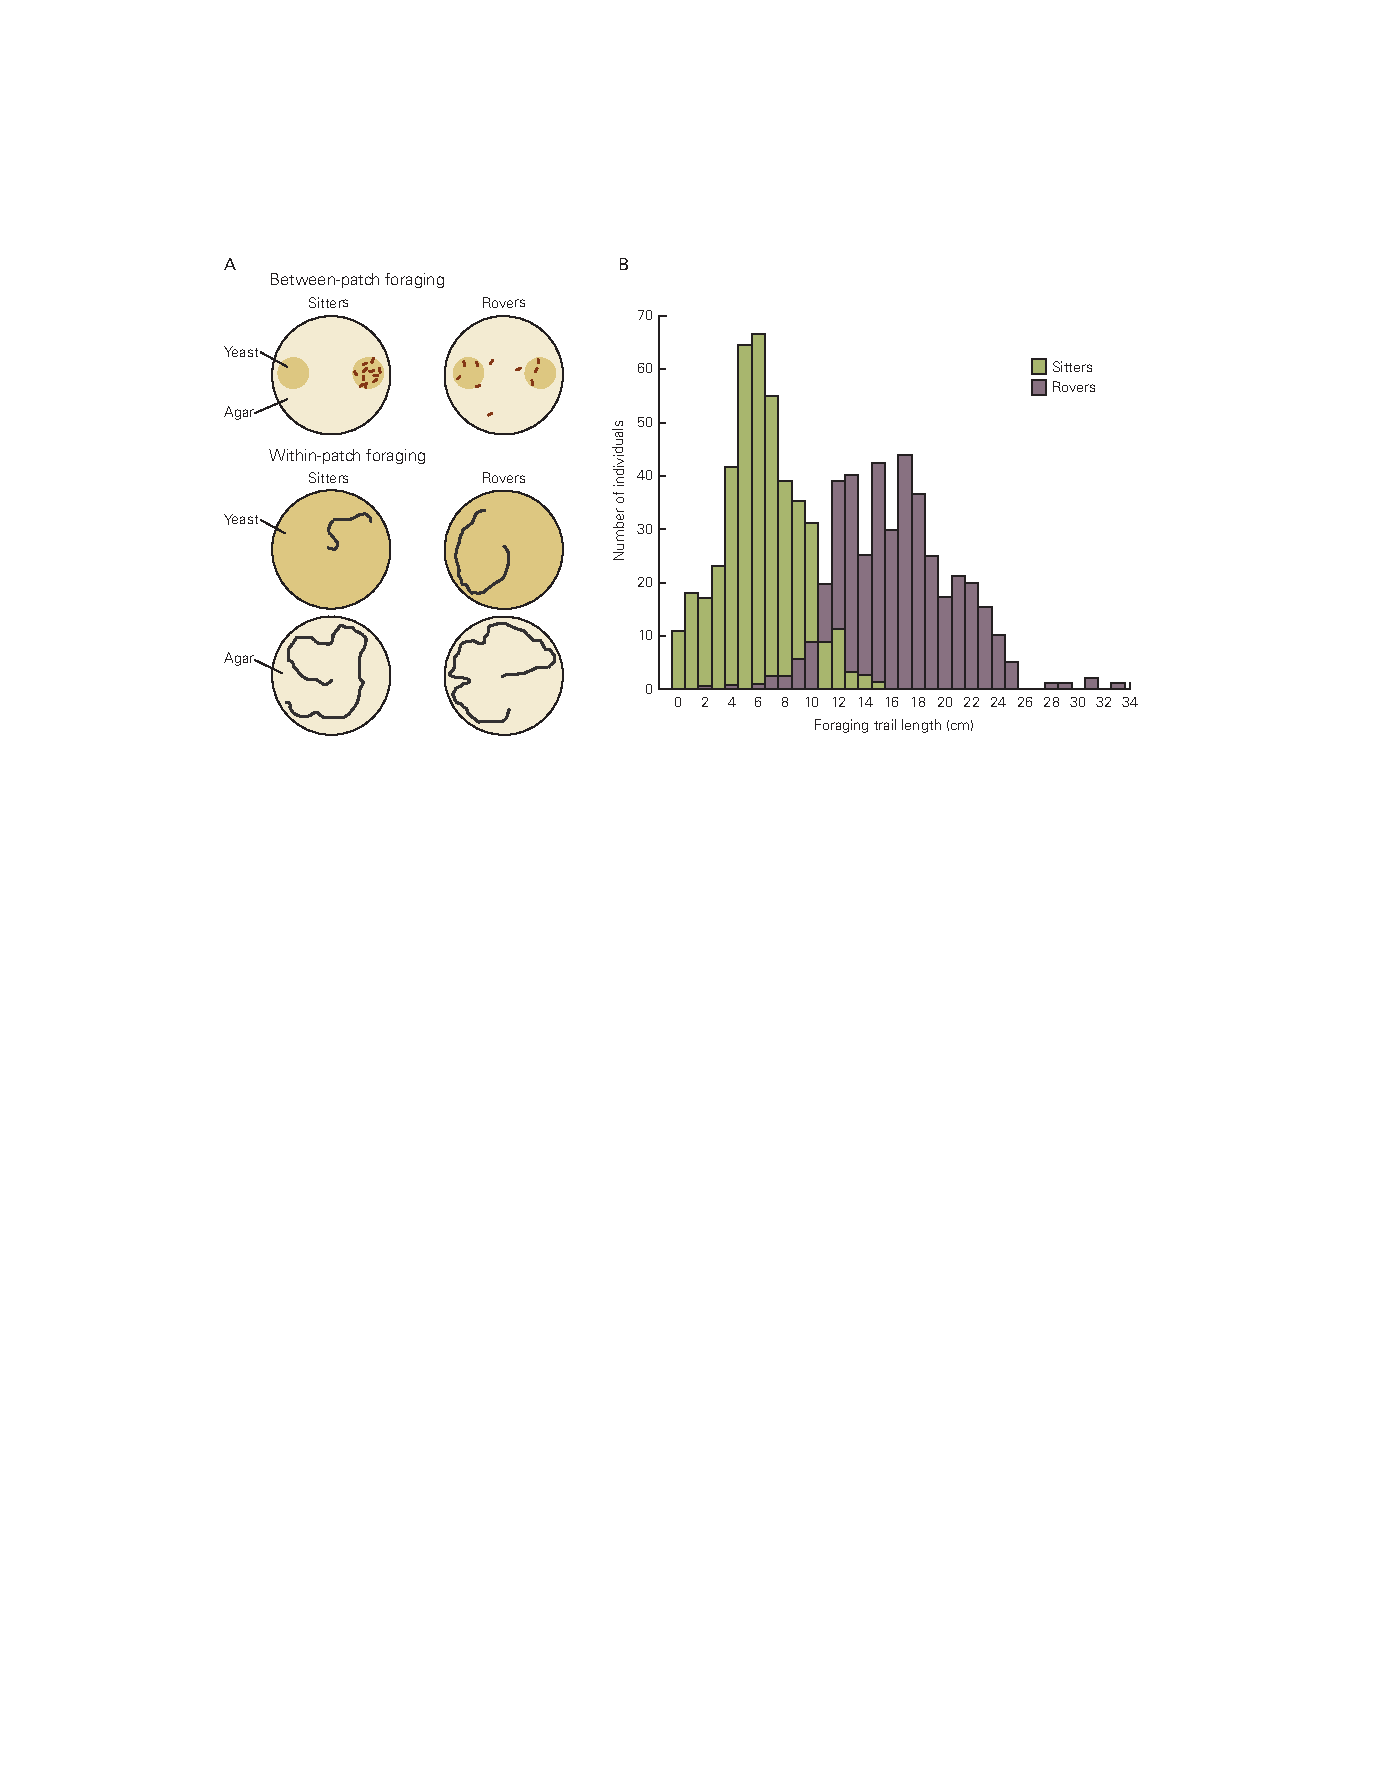
\includegraphics[width=0.5\linewidth]{chap02/fig_2_14}
	\caption{果蝇漫游者和保姆幼虫在享用酵母时的觅食行为不同\cite{sokolowski2001drosophila}。
		\textbf{A.} 漫游型幼虫从一块地移动到另一块地,而保姆型幼虫在一块地上停留很长时间。
		当在一块地里觅食时,漫游者幼虫比保姆幼虫移动得更多。
		仅在琼脂上,漫游者和保姆幼虫的移动速度相等。
		\textbf{B.} 当漫游者在一片食物中觅食时,它们的踪迹长度比坐着的人长(踪迹长度是在5分钟内测量的)。
		这种觅食行为的差异映射到一个单一的蛋白激酶基因,该基因在不同的苍蝇幼虫中的活性不同。}
	\label{fig:2_14}
\end{figure}


Sokolowski 使用不同野生果蝇之间的杂交来研究漫游者和保育幼虫之间的遗传差异。
这些杂交表明漫游者和保育幼虫之间的差异在于一个主要基因,即 for (forager) 基因座。
for 基因编码信号转导酶,一种由细胞代谢物 cGMP(环鸟苷 3',5'-单磷酸)激活的蛋白激酶。
因此,这种行为的自然变化源于信号转导通路调节的改变。
许多神经元功能受蛋白激酶调节,例如由 for 基因编码的 cGMP 依赖性激酶。
蛋白激酶等分子在将短期神经信号转化为神经元或回路特性的长期变化方面尤为重要。


为什么信号酶的变异性会在通常包括漫游者和保育者的果蝇野生种群中得以保留?
答案是环境的变化会产生压力,要求平衡选择替代行为。 
拥挤的环境有利于漫游者幼虫,它能比竞争对手更有效地移动到新的、未开发的食物来源,而稀疏的环境有利于保育幼虫,它能更彻底地利用当前来源。


for 基因也存在于蜜蜂中。
蜜蜂在生命的不同阶段表现出不同的行为;
一般来说,年轻的蜜蜂是护士,而年长的蜜蜂则成为离开蜂巢的觅食者。
for 基因在活跃的觅食蜜蜂的大脑中以高水平表达,而在更年轻和更静止的护士蜜蜂中以低水平表达。
幼蜂中 cGMP 信号的激活会导致它们过早进入觅食阶段;
这种变化可能是由环境刺激或蜜蜂的衰老引起的。


因此,同一个基因控制两种不同昆虫行为的变异,但方式不同。
在果蝇中,行为的变化在不同的个体中表现出来,而在蜜蜂中,它们在不同年龄的个体中表现出来。
这种差异说明了一个重要的调控基因是如何被招募到不同物种的不同行为策略中的。



\subsection{神经肽受体调节几种物种的社会行为}

行为的许多方面都与动物与其他动物的社会互动有关。
社会行为在物种之间变化很大,但在受遗传控制的物种中具有很大的先天组成部分。
在蛔虫秀丽隐杆线虫中分析了一种简单的社会行为形式。 
这些动物生活在土壤中,以细菌为食。


不同的野生型菌株在摄食行为上表现出巨大差异。
来自标准实验室菌株的动物是孤独的,分散在细菌食物的草坪上并且彼此之间无法互动。
其他菌株具有群居摄食模式,加入由数十或数百只动物组成的大型摄食群(图~\ref{fig:2_15})。
这些菌株之间的差异是遗传的,因为这两种喂养方式都是稳定遗传的。


\begin{figure}[htbp]
	\centering
	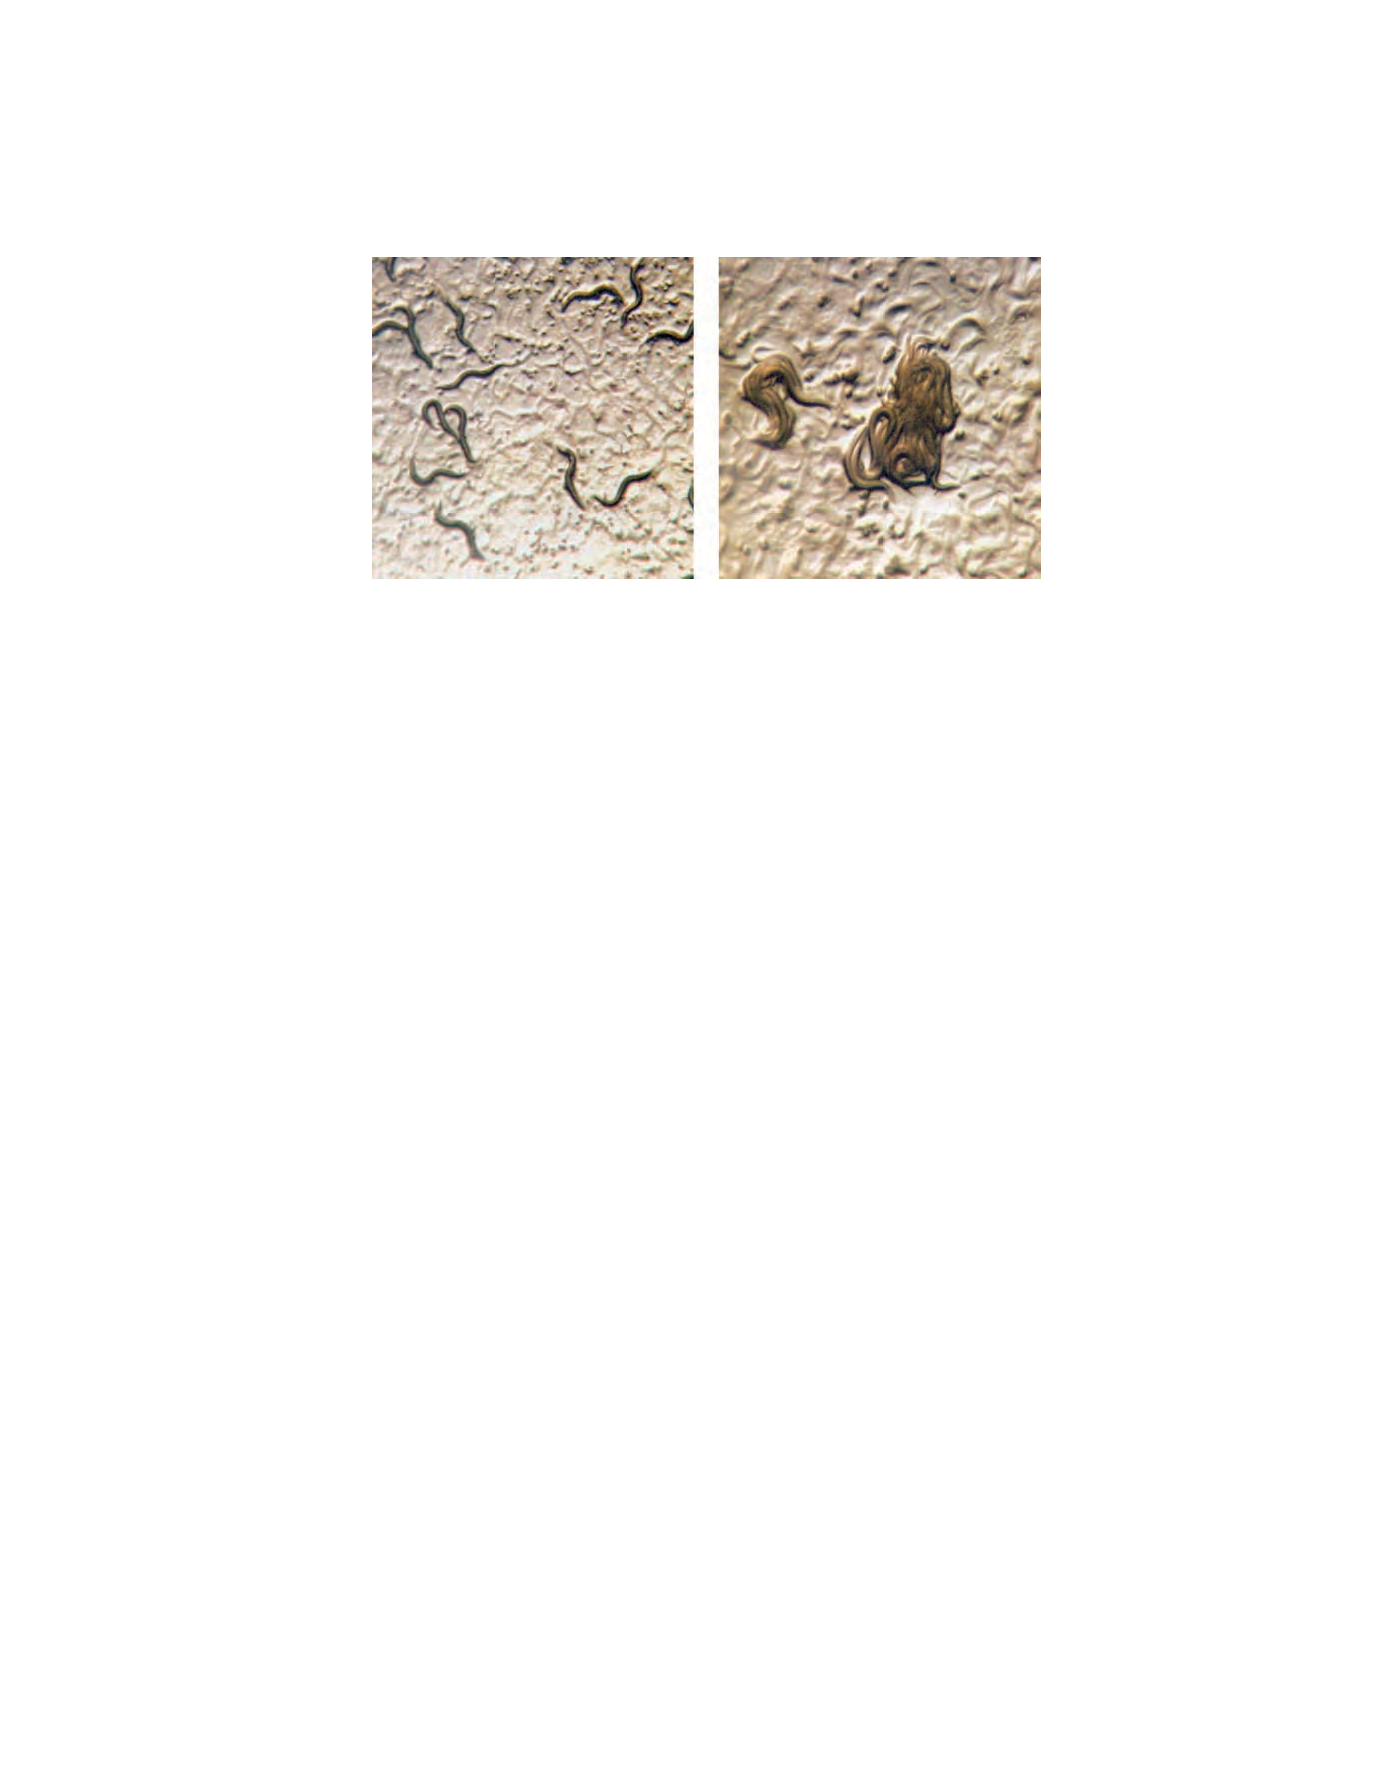
\includegraphics[width=0.5\linewidth]{chap02/fig_2_15}
	\caption{秀丽隐杆线虫的进食行为取决于编码神经肽受体的基因的活性水平。
		在一个菌株中,个体蠕虫在隔离状态下吃草(左),而在另一个菌株,个体聚集在一起觅食。
		这种差异可以通过神经肽受体基因中的单个氨基酸取代来解释\cite{de1998natural}。}
	\label{fig:2_15}
\end{figure}


群居蠕虫和独居蠕虫之间的差异是由单个基因中的单个氨基酸取代引起的,该基因是参与神经元间信号传导的一大基因家族的成员。
该基因 npr-1 编码神经肽受体。
长期以来,神经肽因其在跨神经元网络协调行为方面的作用而受到赞赏。
例如,海蜗牛 Aplysia 的神经肽激素会刺激与单一行为(产卵)相关的一组复杂的运动和行为模式。
哺乳动物神经肽与摄食行为、睡眠、疼痛和许多其他行为和生理过程有关。
改变社会行为的神经肽受体突变的存在表明,这种信号分子对于产生行为和产生个体之间的差异都很重要。


神经肽受体也与哺乳动物社会行为的调节有关。
神经肽催产素和加压素刺激哺乳动物的亲和行为,例如配对结合和父母与后代的结合。
在小鼠中,社会认知需要催产素,即识别熟悉个体的能力。
催产素和加压素已在草原田鼠中进行了深入研究,草原田鼠是一种长期成对抚养幼崽的啮齿动物。
雌性草原田鼠在交配过程中大脑中释放的催产素会刺激配对关系的形成。
同样,雄性草原田鼠在交配过程中大脑中释放的加压素会刺激配对关系的形成和父系行为。


配对结合的程度在哺乳动物物种之间有很大差异。
雄性草原田鼠与雌性形成长期的配偶关系,帮助它们抚养后代,被描述为一夫一妻制,但密切相关的雄性山地田鼠繁殖广泛,不参与父系行为。
这些物种中雄性行为的差异与大脑中 V1a 类加压素受体表达的差异相关。
在草原田鼠中,V1a 加压素受体在特定大脑区域(腹侧苍白球)中以高水平表达(图~\ref{fig:2_16})。 
在山地田鼠中,该区域的水平要低得多,尽管其他大脑区域的水平很高。


\begin{figure}[htbp]
	\centering
	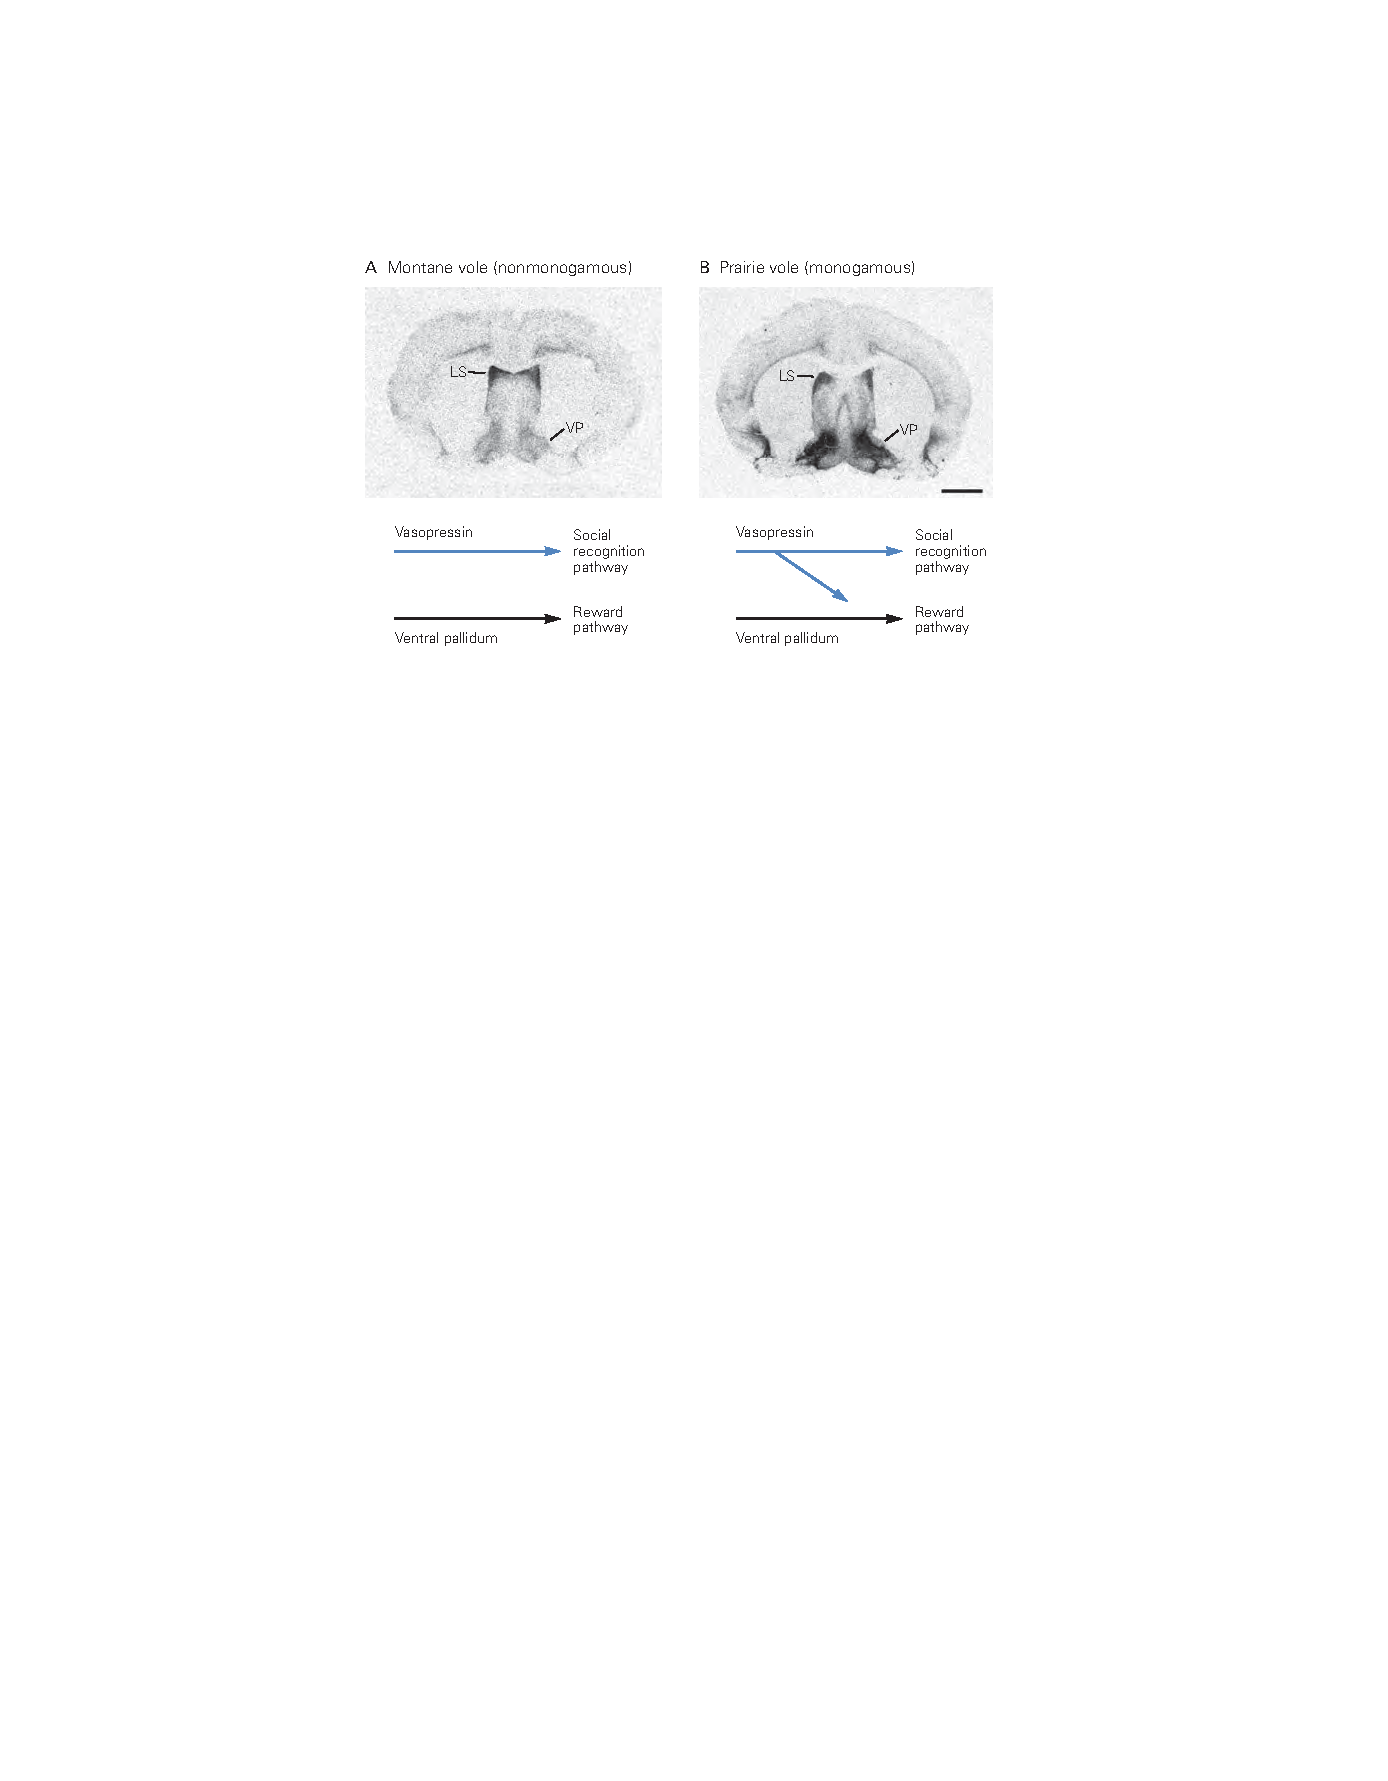
\includegraphics[width=0.5\linewidth]{chap02/fig_2_16}
	\caption{血管加压素受体(V1a)在两种亲缘关系密切的啮齿动物中的分布\cite{young2001cellular}。
		\textbf{A.} 受体在山地田鼠的侧隔膜(LS)中表达较高,但在腹侧苍白球(VP)中表达较低,这不会形成配对键。
		\textbf{B.} 在一夫一妻制草原田鼠的腹侧苍白球中表达很高。
		受体在腹侧苍白球中的表达使加压素将社会识别途径与奖励途径联系起来。}
	\label{fig:2_16}
\end{figure}


催产素和加压素及其受体的重要性已通过小鼠反向遗传研究得到证实和扩展,这比田鼠更容易进行遗传操作。
将草原田鼠的 V1a 加压素受体基因引入行为更像山地田鼠的雄性小鼠,增加了 V1a 加压素受体在腹侧苍白球中的表达,并增加了雄性小鼠对雌性的亲和行为。
因此,物种之间加压素受体表达模式的差异可能导致社会行为的差异。


对不同啮齿动物中加压素受体的分析提供了对基因和行为在进化过程中发生变化的机制的深入了解。
因此,腹侧前脑 V1a 加压素受体表达模式的进化变化改变了神经回路的活动,将腹侧前脑的功能与交配激活的加压素分泌神经元的功能联系起来。
结果,社会行为发生了改变。


催产素和后叶加压素在人类社会行为中的重要性尚不清楚,但配对和幼崽饲养在哺乳动物物种中的核心作用表明这些分子可能也在我们物种中发挥作用。



\section{人类遗传综合症的研究为社会行为的基础提供了初步见解}

\subsection{人类脑部疾病是基因与环境相互作用的结果}

在人类中发现的第一个神经系统疾病基因清楚地说明了基因和环境在决定认知和行为表型方面的相互作用。
苯丙酮尿症 (PKU) 于 1934 年由挪威的 AsbØrn FØlling 描述,影响 15,000 名儿童中的一名,并导致认知功能严重受损。


患有这种疾病的儿童有两个编码苯丙氨酸羟化酶的 PKU 基因的异常拷贝,苯丙氨酸羟化酶是一种将氨基酸苯丙氨酸转化为酪氨酸的酶。
该突变是隐性的,杂合子携带者个体没有任何症状。
该基因的两个拷贝都缺乏正常功能的儿童会从膳食蛋白质中积累高血浓度的苯丙氨酸,这反过来会导致产生干扰神经元功能的有毒代谢物。
苯丙氨酸对大脑产生不利影响的具体生化过程仍不清楚。


PKU 表型(智力障碍)是基因型(纯合子 pku 突变)和环境(饮食)相互作用的结果。
因此,PKU 的治疗简单有效:可以通过低蛋白饮食来预防发育迟缓。
PKU 基因功能的分子和遗传分析已使受影响个体的生活得到显着改善。
自 1960 年代初以来,美国对新生儿 PKU 进行了强制性检测。
在疾病出现之前识别患有遗传疾病的儿童并改变他们的饮食可以预防该疾病的许多方面。


本书后面的章节描述了很多单基因特征的例子,例如 PKU,这些特征导致了对大脑功能和功能障碍的深入了解。
这些研究中出现了某些主题。
例如,许多罕见的神经退行性疾病,如亨廷顿病和脊髓小脑性共济失调,是由蛋白质中谷氨酸残基的病理性显性扩张引起的。
这些多聚谷氨酰胺重复障碍的发现突出了未折叠和聚集的蛋白质对大脑的危险。
癫痫发作可由离子通道中的各种突变引起的发现导致人们认识到这些疾病主要是神经元兴奋性障碍。



\subsection{罕见的神经发育综合症为社会行为、知觉和认知的生物学提供了见解}

在儿童时期表现出来的神经和发育障碍已经阐明了遗传学在人类大脑功能中的重要性和复杂性。
基因影响特定认知和行为回路的早期证据来自对称为威廉姆斯综合征的罕见遗传病症的研究。
患有这种疾病的人通常表现出正常的语言和极端的社交能力;
在发育早期,他们缺乏儿童通常在陌生人面前表现出的沉默寡言。
同时,他们在空间处理方面严重受损,表现出整体智力障碍,并且焦虑率非常高(但很少有社交焦虑症)。


与孤独症谱系障碍等疾病相比,威廉姆斯综合征的损伤模式表明,语言和社交技能可以与其他一些大脑功能区分开来。
与语言有关的大脑区域在孤独症儿童中受损,但在威廉姆斯综合症中活跃或加重。
相比之下,威廉姆斯综合征的一般智力和空间智力受损程度超过所有孤独症谱系障碍儿童的大约一半。


威廉姆斯综合症是由染色体区域 7q11.23 的杂合缺失引起的,通常包含约 1.5 Mb 和 27 个基因。
对该缺陷最简单的解释是,区间内基因的表达水平降低,因为该区域每个基因只有一个拷贝,而不是两个拷贝。
影响社会交流和空间处理的区间中的精确基因尚不清楚,但由于它们有可能提供对人类行为的遗传调控的洞察力,因此引起了极大的兴趣。


孤独症谱系障碍研究的最新发现进一步强调了遗传变异与社会和智力功能之间的复杂关系,这首先是由威廉姆斯综合症阐明的。
大约在过去十年内,基因组技术的进步使高通量方法能够筛选基因组中染色体结构的变异,并且分辨率比光学显微镜高得多(见框 2-1)。
2007 年和 2008 年的开创性研究表明,患有孤独症谱系障碍的个体比未受影响的个体更常携带新的(从头)拷贝数变异。
这些发现导致了一些特定基因组间隔的首次发现,这些间隔导致了该综合征的常见形式(即没有综合征特征证据的孤独症谱系障碍,也称为特发性或非综合征性孤独症谱系障碍)。


2011 年,在一个非常明确的队列中同时开展两项从头拷贝数变异的大规模研究发现,威廉姆斯综合征中删除的恰好相同区域会给个体带来孤独症谱系障碍的重大风险。
然而,在这些情况下,是罕见的重复(该区域的一个多余副本),而不是缺失,大大增加了社会残疾的风险。
这些发现,即同一组基因的损失和获得可能导致截然不同的社会表型(虽然两者通常都会导致智力障碍),进一步支持认知和行为功能领域是可分离的但可能共享重要分子机制的观点。


脆性 X 综合征是另一种儿童神经发育障碍,可以深入了解认知功能的遗传学; 与威廉姆斯综合症不同,它已被映射到 X 染色体上的单个基因。
脆性 X 综合征的表现各不相同。
患儿可有智力障碍、社会认知差、社交焦虑高、行为重复;
大约 30\% 的脆性 X 综合征男孩符合孤独症谱系障碍的诊断标准。
脆性 X 综合征还与更广泛的特征相关,包括身体特征,例如拉长的脸和突出的耳朵。


脆性 X 综合征已被证明是由减少称为脆性 X 智力低下蛋白 (FMRP) 的基因表达的突变引起的。
因为该基因落在 X 染色体上,当男性的一个拷贝发生突变时,男性将失去该基因的所有表达。
FMRP 蛋白在神经元中调节\textit{信使核糖核酸}向蛋白质的翻译,这一过程本身受神经元活动调节。
神经元中受调节的翻译是学习所需的突触可塑性的重要组成部分。
因此,翻译水平上的脆弱 X 缺陷会级联起来影响神经元功能、学习和高级认知过程。
有趣的是,大部分与孤独症谱系障碍和精神分裂症风险增加相关的其他基因都受 FMRP 蛋白调节。


另一种遗传基础广为人知的孟德尔疾病是 Rett 综合征(在第~\ref{chap:chap62}~章中详细讨论)。
Rett 综合征是一种 X 连锁的进行性神经发育障碍,是女性智力障碍的最常见原因之一。
这种疾病几乎总是局限于女性,因为典型的 Rett 突变在发育中的男性胚胎中通常是致命的,而男性胚胎只有一条 X 染色体。
受影响的女孩通常会发育到 6 到 18 个月大,这时她们无法学会说话,智力功能退化,并且表现出强迫性、不受控制的拧手而不是有目的的手部运动。
此外,患有 Rett 综合症的女孩通常会表现出一段时间的社交互动明显受损,这可能与孤独症谱系障碍无法区分,尽管人们认为社交功能在以后的生活中很大程度上得到了保留。
Huda Zoghbi 和她的同事发现,这种综合征的主要原因是甲基 CpG 结合蛋白 2 (MeCP2) 基因的突变。
\textit{脱氧核糖核酸}中特定 CpG 序列的甲基化会改变附近基因的表达,而 MeCP2 的一项既定功能是它结合甲基化\textit{脱氧核糖核酸}作为调节\textit{信使核糖核酸}转录过程的一部分。


罕见综合征还提供了一些对精神分裂症遗传底物的初步见解(第~\ref{chap:chap60}~章)。
例如,正如 Robert Shprintzen 及其同事在 1978 年首次描述的那样,22q11 染色体缺失会导致广泛的身体和行为症状,包括精神病,现在通常被称为心面综合征 (VCFS)、DiGeorge 综合征或 22q11 缺失综合征。
由于与相同缺失相关的表型范围极其广泛,Shprintzen 的最初描述遭到了一些怀疑。
现在人们普遍认为,22q11 缺失是与精神分裂症和儿童期发病的精神分裂症相关的最常见的染色体异常。
此外,已发现同一区域的染色体丢失与孤独症的个体风险有关。
迄今为止,尚未明确确定该区域内负责精神病表型的特定基因。
此外,最近来自孤独症文献的证据表明,很可能是这个区间内多个基因的组合,每个基因赋予相对较小的个体影响,是社会残疾表型的原因。



\section{精神疾病涉及多基因特征}

如前所述,与神经退行性疾病和精神疾病的总负担相比,单基因综合征很少见。
因此,如果罕见疾病仅占总疾病负担的一小部分,人们可能会质疑研究罕见疾病的理由。
原因是罕见的情况可以让人们深入了解更常见、更复杂的疾病形式所涉及的生物学过程。
例如,人类遗传学取得的突出成就之一是发现了导致早发性阿尔茨海默病或帕金森病的罕见基因变异。
具有这些严重罕见变异的个体代表了所有患有这些疾病的个体的一小部分,但对罕见疾病变异的鉴定揭示了在更大的患者群体中也被破坏的细胞过程,指向了一般的治疗途径。
同样,对 Rett、脆性 X 和其他神经发育障碍背后的病理生理机制的探索已经导致了对精神综合症合理药物开发的一些初步尝试。


在本章的其余部分,我们将进一步讨论两种复杂的神经发育和精神病表型的遗传学:孤独症谱系障碍和精神分裂症。
与前面讨论的罕见孟德尔例子相比,这些疾病的常见形式的遗传学确实更加多样化、多样和异质,涉及不同个体的许多不同基因以及赋予责任的多种风险基因组合。
此外,对于这两种诊断,虽然对遗传贡献的支持是巨大的,但也有令人信服的证据表明环境因素的贡献。


理解这些疾病的进展来自快速发展的基因组技术和统计方法的结合、开放数据共享的文化以及非常大的患者队列的整合,这些患者队列提供了足够的能力来检测非常罕见的高渗透性等位基因以及携带的常见遗传变异 风险的小增量。
重要的是,最近在理解这两种综合征方面取得的成功为研究它们的生物学后果以及这些遗传风险因素所传达的分子、细胞和回路级病理生理学提供了坚实的基础。



\subsection{孤独症谱系障碍遗传学的进展突出了罕见和从头突变在神经发育障碍中的作用}

孤独症谱系障碍是一组严重程度不同的发育综合症,影响大约 2\% 至 3\% 的人口,其特征是相互社会交流障碍以及刻板兴趣和重复行为。
男性明显占优势;
平均而言,受影响的男孩是女孩的三倍。
孤独症谱系障碍的临床症状,根据定义,出现在生命的前 3 年,尽管受影响和未受影响的儿童之间高度可靠的差异通常在生命的头几个月内可以识别。


受影响的人之间存在相当大的表型变异性,导致孤独症谱系障碍的诊断分类相当广泛。
此外,受影响的个体比一般人群更容易出现癫痫发作和认知问题,并且通常在适应功能方面存在严重障碍。
然而,许多孤独症患者并没有受到如此深远的影响,并过着非常成功的生活。


孤独症具有很强的遗传成分(见图~\ref{fig:2_1}A),这很可能解释了它是首批屈服于现代基因发现工具和方法的遗传复杂神经精神综合征之一。
孤独症谱系障碍具有更广泛的意义,因为它提供了对典型人类行为的洞察力:语言、复杂智力和人际互动。
重要的是,孤独症谱系障碍中的社交沟通缺陷可以与其他领域的正常智力和典型功能共存,这一事实表明大脑在某种程度上是模块化的,具有可以独立变化的不同认知功能。


虽然孤独症谱系障碍的综合征形式只占所有病例的一小部分,但在更常见的所谓“特发性”或“非综合征”形式的障碍中的首次发现也证明了罕见突变的作用,这些突变具有巨大的生物学效应。
例如,在 2003 年,对极少数具有孤独症特征的女性 X 染色体上缺失区域的基因进行测序,导致在基因 neuroligin 4X (NLGN4X) 中发现了罕见的功能丧失突变, 一种在兴奋性神经元中编码突触粘附分子的基因,在几个受影响的男性家庭成员中发现。
此后不久,对一个患有智力障碍和孤独症谱系障碍的大型家系进行的连锁分析表明,受影响的家庭成员都携带功能丧失型 NLGN4X 突变。


染色体结构中的从头亚显微缺失和重复可能会显着增加个体患孤独症谱系障碍的风险。
这些拷贝数变异 (CNV) 聚集在基因组的特定区域,确定特定的风险区间。 使用这种方法的最早报告表明,染色体 16p11.2 的新生 CNV,虽然仅存在于大约 0.5\% 至 1\% 的受影响个体中,但具有很大(大于 10 倍)的孤独症谱系障碍风险。
随后的研究现在已经确定了十几个或更多具有风险的新 CNV,包括染色体 16p11.2、1q21、15q11-13 和 3q29; 22q11、22q13(删除基因 SHANK3)和 2p16(删除基因 NXRN1)的缺失;和 7q11.23(Williams 综合征区域)的从头重复。


有趣的是,尽管这些 CNV 对孤独症谱系障碍具有很大的风险,但对其他精神疾病(包括精神分裂症和双相情感障碍)的研究发现,许多相同的区域也会增加患这些疾病的风险。
此外,通过基因型(例如,16p11.2 缺失和重复)确定的个体研究发现了多种相关的行为表型,从特定语言障碍到智力障碍再到精神分裂症。
这种“一对多”现象对阐明精神疾病的特定病理生理机制以及概念化从基因发现到治疗的步骤提出了重要挑战。


从头开始的罕见 CNV 会增加孤独症谱系障碍和其他发育障碍的风险,这一广泛且可复制的发现立即引发了一个问题,即单个基因中的罕见从头突变是否可能带来类似的风险。
事实上,低成本、高通量\textit{脱氧核糖核酸}测序技术的发展,最初侧重于基因组的编码部分,导致在受影响的基因组中发现了被认为可能破坏基因功能(LGD 突变)的过量从头突变。
个人。
这些突变在不相关的个体之间近距离反复发生,现已被用作识别孤独症谱系障碍特定风险基因的手段。


对孤独症谱系障碍新生突变的大规模研究现已确定了 100 多个相关基因,其中约 45 个达到统计显着性的最高置信水平。
这些基因具有广泛的已知功能,但分析显示参与突触形成和功能以及转录调节的基因在统计学上显着过度表达。
此外,编码\textit{核糖核酸}的风险基因数量超过预期,这些\textit{核糖核酸}是脆性 X 智力低下蛋白和/或在早期大脑发育中活跃的蛋白质的目标。



\subsection{精神分裂症基因的鉴定突出了罕见和常见风险变异的相互作用}

精神分裂症影响了大约 1\% 的年轻人,导致思维障碍和情绪退缩的模式,严重损害了生活。
它具有很强的遗传性(参见图~\ref{fig:2_1}B),并且还具有与发育中胎儿的压力相关的强大环境成分。
二战荷兰饥饿冬季饥荒后不久出生的儿童在多年后患精神分裂症的风险大大增加,而母亲在 1960 年代大流行期间怀孕期间感染风疹病毒的儿童的风险也大大增加。


基因和环境都会导致精神分裂症。
与孤独症一样,人类基因组的测序、常见变异的全基因组基因分型和 CNV 检测的廉价方法的开发,以及非常大的患者队列的整合,都导致了精神分裂症遗传学的转变。
首先,与早先提到的孤独症谱系障碍的发现基本平行,到 2000 年代初期,罕见的新发 CNV 开始与精神分裂症的风险有关。
一小部分病例与具有较大风险的染色体异常有关,例如,染色体 22q11 的缺失。
这些染色体异常与孤独症谱系障碍相关的基因座完全或几乎重叠,但这些基因座缺失和重复的风险分布似乎并不相同。
例如,虽然 16p11.2 区域的重复和缺失都与孤独症谱系障碍和精神分裂症有关,但该区域的重复更有可能导致精神分裂症,而缺失更可能与孤独症谱系障碍和智力障碍相关。


关于精神分裂症,过去十五年来最重要的发展是常见变异全基因组关联研究的出现。
与前面描述的假设驱动的候选基因研究相反,全基因组关联依赖于同时检测基因组中每个基因的多态性。
这种无假设的方法,当与有力的队列一起使用并适当校正多重比较时,已被证明是一种高度可靠和可重复的策略,用于识别所有医学常见疾病中的常见风险等位基因。


涉及近 40,000 个病例和 113,000 个对照的全基因组关联研究已经确定了 108 个精神分裂症的风险位点。 
这组中任何个体遗传变异的影响都非常适度,通常导致风险增加不到 25\%。
此外,在全基因组关联研究中测定的许多遗传多态性映射到基因组编码区段之外的区域。
因此,虽然已经确定了 108 个风险基因座,但尚不完全清楚哪些基因对应于所有这些风险变异。
在某些情况下,变异与单个基因的映射足够接近,可以合理地推断出这种关系;
在其他情况下,这仍有待确定。


与精神分裂症风险有关的基因为确定该疾病的生物学基础提供了一个起点。
例如,自 20 世纪 90 年代后期以来,有证据表明一个叫做主要组织相容性复合体 (MHC) 的区域与精神分裂症风险有关。
因此,在精神分裂症队列中,MHC 区域具有人类基因组任何部分中最强的全基因组关联研究信号。
队列中的大量患者使详细研究成为可能,将 MHC 区域中的这种强大的风险关联信号解析为三个不同的基因座(可能是三个不同的基因)。
在这三个基因座中,一个编码补体 C4 因子的基因对疾病风险具有强烈且明确的影响。
Steven McCarroll 和他的同事表明,补体 C4 基因座代表 CNV 的自然病例,健康个体在他们拥有的基因拷贝数方面存在很大差异,并且 C4A 等位基因的表达水平与精神分裂症风险的增加相关。
随后的后续研究表明,敲除 C4 基因的小鼠在发育过程中存在突触修剪缺陷,这表明人类 C4A 过量可能导致突触修剪过度的假设,这一过程长期以来一直受到精神分裂症文献的关注。


这一发现代表了将基因组学与增加疾病风险的可能生物学机制联系起来的能力的重要证明。
即便如此,具有最高风险 C4 单倍型且没有精神分裂症家族史的个体会由于该等位基因而平均受影响的几率从 1\% 增加到大约 1.3\%。
为了获得规模感,一级亲属患有精神分裂症会导致患病风险增加约 10 倍。
这一充满希望的开端及其局限性反映了遗传学家和神经生物学家在从成功的常见变异基因发现转向详细阐述导致人类病理学的特定机制方面所面临的挑战。


除了确定许多特定的风险位点外,精神分裂症的\textit{全基因组关联研究}还反复发现许多常见等位基因的小个体效应加起来会增加风险。
这些结果为总体研究基因型表型关系提供了一个额外的、强大的途径。
事实上,已经清楚的是,个体携带的风险等位基因的数量会对患这种疾病的风险产生重大(和累加)影响。
例如,那些在所谓的多基因风险评分(与个人携带的加性遗传风险总量相关的汇总统计数据)中处于最高十分位的人,与一般人群相比,风险增加了 8 到 20 倍。
尽管累积效应的生物学特性尚不清楚,但该观察结果为研究与疾病轨迹和治疗反应相关的一系列有趣问题奠定了基础,并且几乎肯定会重振结合神经影像学和基因组学的研究。
后一种类型的调查,类似于常见变异发现的早期努力,由于研究选定的、生物学上合理的候选基因的固有局限性,可靠性较差。


最后,类似于孤独症谱系障碍所采用的高通量测序方法,也开始在精神分裂症中产生结果。
具体来说,寻找稀有和从头风险等位基因的外显子组测序已经取得了一些成功。
然而,与孤独症谱系障碍相比,此类研究需要更大的队列来确定 LGD 突变的统计学显着风险,这表明这些类型变异的总体影响大小在精神分裂症中可能要小得多。
迄今为止,这些调查已经确定了一些风险基因并涉及关键的神经生物学途径。
特别是,最近的外显子组研究指出了活性调节细胞骨架 (ARC) 复合体中分子的重要性,以及包含 1A (SETDIA) 的基因组结构域,与精神分裂症发病机制相关。



\section{神经精神疾病遗传基础的观点}

基因影响行为的许多方面。 
人类双胞胎在人格特征和精神疾病方面有着显着的相似之处,即使是分开抚养的双胞胎也是如此。 
可以培育具有特定、稳定行为特征的家畜和实验室动物; 
并且越来越多地发现了广泛的遗传变异对神经发育和精神疾病的贡献。


一系列平行的进步开创了一个理解基因、大脑和行为之间关系的绝佳机会的时代。 
可用于操作和研究模型系统的武器库已经发生了革命性的变化。 
与此同时,在确定人类神经精神疾病的遗传风险因素方面取得了长足的进步。 
尽管该领域在此过程中仍处于早期阶段,但已经出现了成功发现基因及其应用于深入生物学理解的价值的多个例子。


最近对神经发育和精神疾病的遗传学研究的许多惊人发现之一是跨越广泛诊断边界的遗传风险重叠。 
虽然生物学不遵循分类诊断标准可能并不令人惊讶,但考虑该领域如何追踪这些影响并得出新的治疗策略仍然是一个巨大的概念挑战。


此外,值得注意的是,对于许多其他尚未看到先前提到的进展类型的精神疾病,计算很简单:更大的投资和更大的样本量将带来更深入的洞察力。 
例如,最近对图雷特综合征和强迫症的新生突变的研究清楚地表明,鉴定高置信度风险基因的限速因素是亲子三重奏测序的可用性。 
同样,重度抑郁症的\textit{全基因组关联研究}研究直到最近才达到足以确认具有统计学意义的相关常见变异的样本量。 
这些研究包括了数十万人,并且毫不奇怪地发现了具有非常小的个体影响的风险等位基因。


最后一点强调了一种想法,即一种尺寸并不适合所有行为、发育和精神疾病的基因组学。 
从模型系统的研究,到罕见孟德尔疾病的阐明,再到解开导致常见疾病的常见和罕见变异,当今可用的工具和机会是前所未有的。 
未来几年应该会深入了解精神疾病和神经发育障碍的生物学,或许还有可能帮助患者及其家人的疗法。


\section{亮点}

1. 脆性 X 综合征、雷特综合征和威廉姆斯综合征等罕见遗传综合征为复杂人类行为的分子机制提供了重要见解。 
此外,虽然仍有大量工作要做,但对这些综合征的研究已经挑战了相关认知和行为缺陷是不可改变的观念,并证明了广泛的模型系统在阐明保守生物学机制方面的效用。


2. 人类基因组测序、高通量基因组分析的发展以及同步计算和方法学的进步导致对人类行为和精神疾病遗传学的理解发生了深刻变化。 
包括精神分裂症和孤独症在内的几种典型疾病已经取得了显着进展,导致鉴定出数十个明确的风险基因和染色体区域。


3. 过去十年精神病学遗传学和基因组学领域的成熟揭示了测试预先指定的候选基因的脆弱性。 
这些类型的研究现在已被常见和稀有等位基因的全基因组扫描所取代。 
再加上严格的统计框架和共识统计阈值,这些正在产生高度可靠和可重复的结果。


4. 目前,累积的证据表明,各种遗传变异构成复杂行为综合征的基础,包括常见和罕见、传播和新生、种系和体细胞、序列和染色体结构变异。 
然而,这些不同类型的遗传变化的相对贡献因特定疾病而异。


5. 人类行为遗传学最新进展的一个惊人发现是具有不同症状和自然史的综合征的遗传风险重叠。 
了解相同的突变如何以及为什么会在不同个体中导致高度不同的表型结果将是未来的主要挑战。


6. 对常见精神疾病的研究结果表明遗传异质性极高。 
这一点,再加上迄今为止已确定的风险基因的生物学多效性,以及人类大脑发育的动态性和复杂性,都表明在从对风险基因的理解转向对行为的理解方面面临着重大挑战。 
同样,目前,阐明风险基因的生物学和揭示行为综合症的病理生理学之间存在重要区别。

%\section{术语表}

%\section{选读}




